% Options for packages loaded elsewhere
\PassOptionsToPackage{unicode}{hyperref}
\PassOptionsToPackage{hyphens}{url}
%
\documentclass[
]{article}
\usepackage{amsmath,amssymb}
\usepackage{iftex}
\ifPDFTeX
  \usepackage[T1]{fontenc}
  \usepackage[utf8]{inputenc}
  \usepackage{textcomp} % provide euro and other symbols
\else % if luatex or xetex
  \usepackage{unicode-math} % this also loads fontspec
  \defaultfontfeatures{Scale=MatchLowercase}
  \defaultfontfeatures[\rmfamily]{Ligatures=TeX,Scale=1}
\fi
\usepackage{lmodern}
\ifPDFTeX\else
  % xetex/luatex font selection
\fi
% Use upquote if available, for straight quotes in verbatim environments
\IfFileExists{upquote.sty}{\usepackage{upquote}}{}
\IfFileExists{microtype.sty}{% use microtype if available
  \usepackage[]{microtype}
  \UseMicrotypeSet[protrusion]{basicmath} % disable protrusion for tt fonts
}{}
\makeatletter
\@ifundefined{KOMAClassName}{% if non-KOMA class
  \IfFileExists{parskip.sty}{%
    \usepackage{parskip}
  }{% else
    \setlength{\parindent}{0pt}
    \setlength{\parskip}{6pt plus 2pt minus 1pt}}
}{% if KOMA class
  \KOMAoptions{parskip=half}}
\makeatother
\usepackage{xcolor}
\usepackage[margin=1in]{geometry}
\usepackage{longtable,booktabs,array}
\usepackage{calc} % for calculating minipage widths
% Correct order of tables after \paragraph or \subparagraph
\usepackage{etoolbox}
\makeatletter
\patchcmd\longtable{\par}{\if@noskipsec\mbox{}\fi\par}{}{}
\makeatother
% Allow footnotes in longtable head/foot
\IfFileExists{footnotehyper.sty}{\usepackage{footnotehyper}}{\usepackage{footnote}}
\makesavenoteenv{longtable}
\usepackage{graphicx}
\makeatletter
\def\maxwidth{\ifdim\Gin@nat@width>\linewidth\linewidth\else\Gin@nat@width\fi}
\def\maxheight{\ifdim\Gin@nat@height>\textheight\textheight\else\Gin@nat@height\fi}
\makeatother
% Scale images if necessary, so that they will not overflow the page
% margins by default, and it is still possible to overwrite the defaults
% using explicit options in \includegraphics[width, height, ...]{}
\setkeys{Gin}{width=\maxwidth,height=\maxheight,keepaspectratio}
% Set default figure placement to htbp
\makeatletter
\def\fps@figure{htbp}
\makeatother
\setlength{\emergencystretch}{3em} % prevent overfull lines
\providecommand{\tightlist}{%
  \setlength{\itemsep}{0pt}\setlength{\parskip}{0pt}}
\setcounter{secnumdepth}{-\maxdimen} % remove section numbering
\ifLuaTeX
  \usepackage{selnolig}  % disable illegal ligatures
\fi
\usepackage{bookmark}
\IfFileExists{xurl.sty}{\usepackage{xurl}}{} % add URL line breaks if available
\urlstyle{same}
\hypersetup{
  pdftitle={Ácidos orgánicos},
  hidelinks,
  pdfcreator={LaTeX via pandoc}}

\title{Ácidos orgánicos}
\author{}
\date{\vspace{-2.5em}}

\begin{document}
\maketitle

{
\setcounter{tocdepth}{2}
\tableofcontents
}
\section{Acidos orgánicos en peso
fresco}\label{acidos-orguxe1nicos-en-peso-fresco}

Concentración del perfíl de ácidos orgánicos a distintos estados de
Madurez

\begin{center}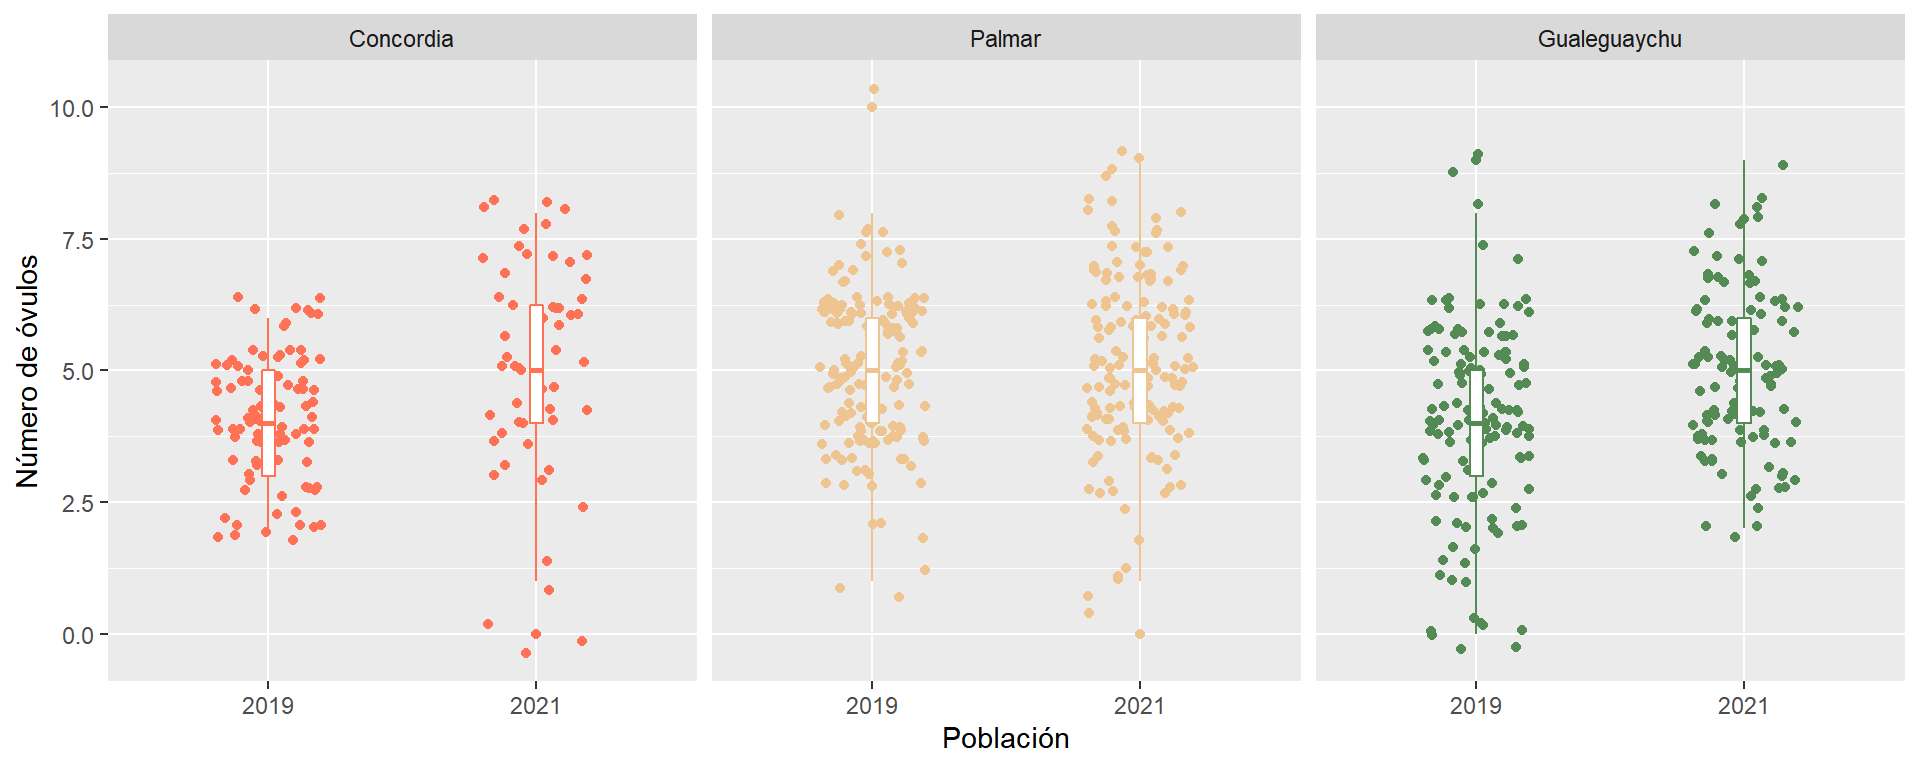
\includegraphics[width=0.95\linewidth]{madAcids_files/figure-latex/unnamed-chunk-2-1} \end{center}

Tabla descriptiva

\begin{longtable}[]{@{}
  >{\raggedright\arraybackslash}p{(\columnwidth - 12\tabcolsep) * \real{0.1515}}
  >{\raggedright\arraybackslash}p{(\columnwidth - 12\tabcolsep) * \real{0.0606}}
  >{\raggedleft\arraybackslash}p{(\columnwidth - 12\tabcolsep) * \real{0.0455}}
  >{\raggedleft\arraybackslash}p{(\columnwidth - 12\tabcolsep) * \real{0.1970}}
  >{\raggedleft\arraybackslash}p{(\columnwidth - 12\tabcolsep) * \real{0.1818}}
  >{\raggedleft\arraybackslash}p{(\columnwidth - 12\tabcolsep) * \real{0.1818}}
  >{\raggedleft\arraybackslash}p{(\columnwidth - 12\tabcolsep) * \real{0.1818}}@{}}
\toprule\noalign{}
\begin{minipage}[b]{\linewidth}\raggedright
CAR
\end{minipage} & \begin{minipage}[b]{\linewidth}\raggedright
MAD
\end{minipage} & \begin{minipage}[b]{\linewidth}\raggedleft
N
\end{minipage} & \begin{minipage}[b]{\linewidth}\raggedleft
CONF
\end{minipage} & \begin{minipage}[b]{\linewidth}\raggedleft
sd
\end{minipage} & \begin{minipage}[b]{\linewidth}\raggedleft
se
\end{minipage} & \begin{minipage}[b]{\linewidth}\raggedleft
ci
\end{minipage} \\
\midrule\noalign{}
\endhead
\bottomrule\noalign{}
\endlastfoot
Tartárico & I & 6 & 0.000000000 & 0.000000000 & 0.000000000 &
0.000000000 \\
Tartárico & MM & 6 & 0.000000000 & 0.000000000 & 0.000000000 &
0.000000000 \\
Tartárico & M & 6 & 0.000000000 & 0.000000000 & 0.000000000 &
0.000000000 \\
Tartárico & SM & 6 & 0.115256167 & 0.056458865 & 0.023049235 &
0.059249945 \\
Málico & I & 6 & 7.387488667 & 2.390397202 & 0.975875571 &
2.508568017 \\
Málico & MM & 6 & 10.975546167 & 0.732827314 & 0.299175498 &
0.769055101 \\
Málico & M & 6 & 11.759538667 & 0.362052545 & 0.147807333 &
0.379950845 \\
Málico & SM & 6 & 10.536866833 & 0.856124888 & 0.349511522 &
0.898447970 \\
Quínico & I & 6 & 0.066569333 & 0.103128768 & 0.042102143 &
0.108227004 \\
Quínico & MM & 6 & 3.076024167 & 0.452481056 & 0.184724617 &
0.474849746 \\
Quínico & M & 6 & 2.545536167 & 0.339503763 & 0.138601831 &
0.356287349 \\
Quínico & SM & 6 & 2.849149333 & 0.498337071 & 0.203445257 &
0.522972683 \\
Succínico & I & 6 & 19.183774833 & 2.084913315 & 0.851162297 &
2.187982339 \\
Succínico & MM & 6 & 11.252415500 & 0.774289201 & 0.316102243 &
0.812566683 \\
Succínico & M & 6 & 11.112724833 & 0.255429687 & 0.104278733 &
0.268057017 \\
Succínico & SM & 6 & 14.317510333 & 0.977555462 & 0.399085346 &
1.025881542 \\
ATT & I & 3 & 1.779200000 & 0.050798425 & 0.029328484 & 0.126190284 \\
ATT & MM & 3 & 1.606400000 & 0.027896953 & 0.016106313 & 0.069299874 \\
ATT & M & 3 & 1.828266667 & 0.203906384 & 0.117725406 & 0.506531538 \\
ATT & SM & 3 & 1.384533333 & 0.083527560 & 0.048224659 & 0.207493963 \\
TOTALac & I & 6 & 26.637833026 & 1.990422196 & 0.812586459 &
2.088819991 \\
TOTALac & MM & 6 & 25.303985619 & 1.788299304 & 0.730070134 &
1.876705024 \\
TOTALac & M & 6 & 25.417799690 & 0.434146910 & 0.177239734 &
0.455609240 \\
TOTALac & SM & 6 & 27.818782698 & 1.061812720 & 0.433483228 &
1.114304111 \\
NA & I & 6 & 45.629847833 & 4.811537003 & 1.964301756 & 5.049398414 \\
NA & MM & 6 & 36.768222667 & 5.141035970 & 2.098819146 & 5.395186373 \\
NA & M & 6 & 39.159253500 & 2.599418000 & 1.061207955 & 2.727921892 \\
NA & SM & 6 & 53.119642833 & 1.842284749 & 0.752109600 & 1.933359275 \\
\end{longtable}

Evolución del perfíl de ácidos orgánicos

\begin{verbatim}
## Error in `palette()`:
## ! Insufficient values in manual scale. 6 needed but only 4 provided.
\end{verbatim}

\subsection{Acidos orgánicos Totales}\label{acidos-orguxe1nicos-totales}

Concentración de ácidos orgánicos totales

\begin{center}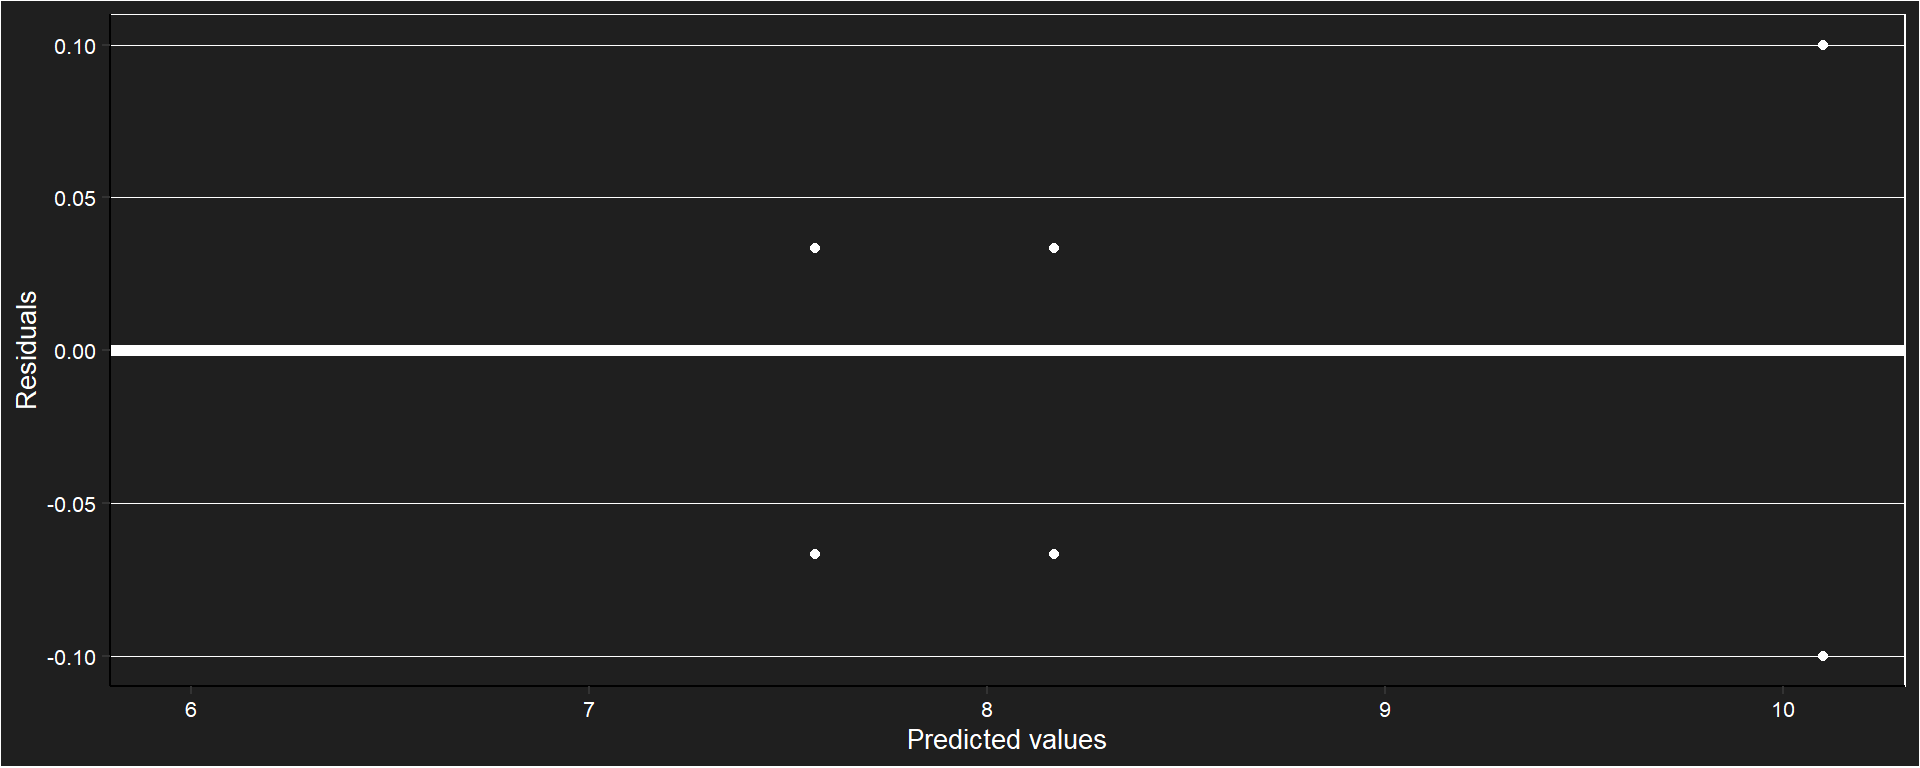
\includegraphics[width=0.95\linewidth]{madAcids_files/figure-latex/unnamed-chunk-6-1} \end{center}

Tabla descriptiva totales

\begin{longtable}[]{@{}llrrrrr@{}}
\toprule\noalign{}
CAR & MAD & N & TOTALF & sd & se & ci \\
\midrule\noalign{}
\endhead
\bottomrule\noalign{}
\endlastfoot
ACIDS & I & 6 & 26.63783300 & 1.990422128 & 0.812586431 & 2.088819919 \\
ACIDS & MM & 6 & 25.30398550 & 1.788299193 & 0.730070088 &
1.876704908 \\
ACIDS & M & 6 & 25.41779983 & 0.434147222 & 0.177239861 & 0.455609568 \\
ACIDS & SM & 6 & 27.81878267 & 1.061812544 & 0.433483156 &
1.114303926 \\
CATIONS & I & 3 & 3.59063333 & 1.325520714 & 0.765289741 &
3.292775993 \\
CATIONS & MM & 3 & 2.56066667 & 0.313536989 & 0.181020665 &
0.778869058 \\
CATIONS & M & 3 & 2.60383333 & 0.308997643 & 0.178399872 &
0.767592698 \\
CATIONS & SM & 3 & 2.21436667 & 0.394508331 & 0.227769491 &
0.980013023 \\
STAT & I & 3 & 1.72112248 & 0.263331774 & 0.152034671 & 0.654152390 \\
STAT & MM & 3 & 1.44765169 & 0.116290944 & 0.067140608 & 0.288882719 \\
STAT & M & 3 & 1.54171590 & 0.132691311 & 0.076609364 & 0.329623489 \\
STAT & SM & 3 & 1.90950428 & 0.007733365 & 0.004464861 & 0.019210744 \\
SUGARS & I & 6 & 45.62984817 & 4.811537421 & 1.964301927 &
5.049398853 \\
SUGARS & MM & 6 & 36.76822233 & 5.141036221 & 2.098819248 &
5.395186636 \\
SUGARS & M & 6 & 39.15925367 & 2.599418252 & 1.061208058 &
2.727922157 \\
SUGARS & SM & 6 & 53.11964317 & 1.842284986 & 0.752109696 &
1.933359523 \\
\end{longtable}

\begin{verbatim}
## Linear mixed-effects model fit by REML
##   Data: dataAT 
##   Log-restricted-likelihood: -39.0996772
##   Fixed: TOTALF ~ MAD 
## (Intercept)       MADMM        MADM       MADSM 
## 26.63783300 -1.33384750 -1.22003317  1.18094967 
## 
## Random effects:
##  Formula: ~1 | REP
##         (Intercept)   Residual
## StdDev: 0.544428081 1.37176539
## 
## Number of Observations: 24
## Number of Groups: 3
\end{verbatim}

\begin{center}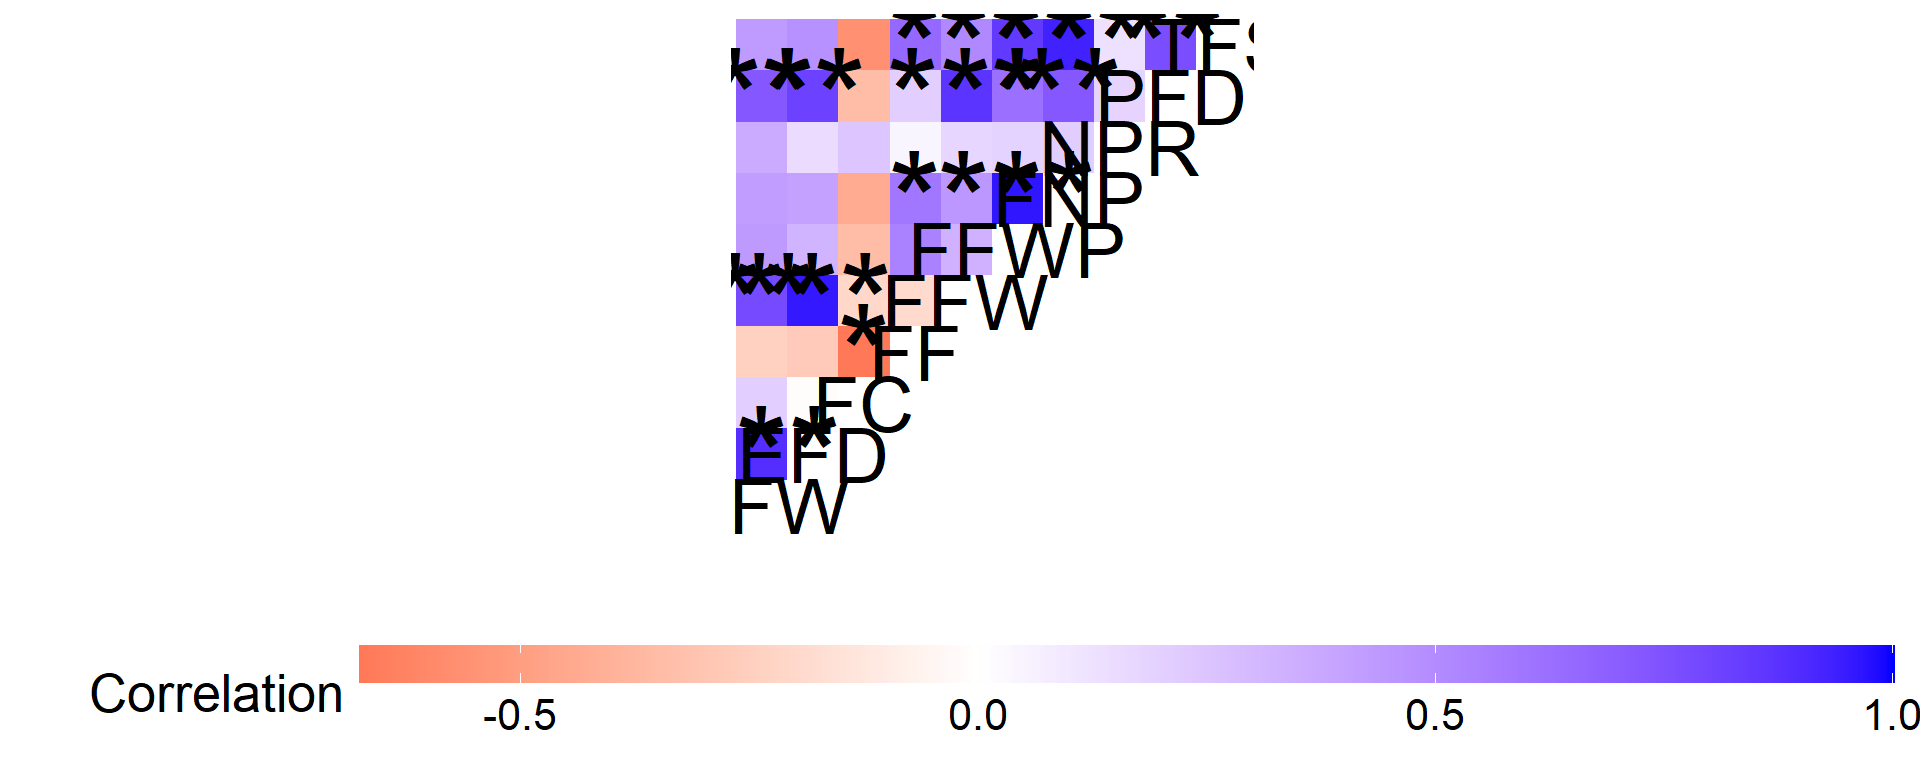
\includegraphics[width=0.95\linewidth]{madAcids_files/figure-latex/unnamed-chunk-8-1} \end{center}

\begin{center}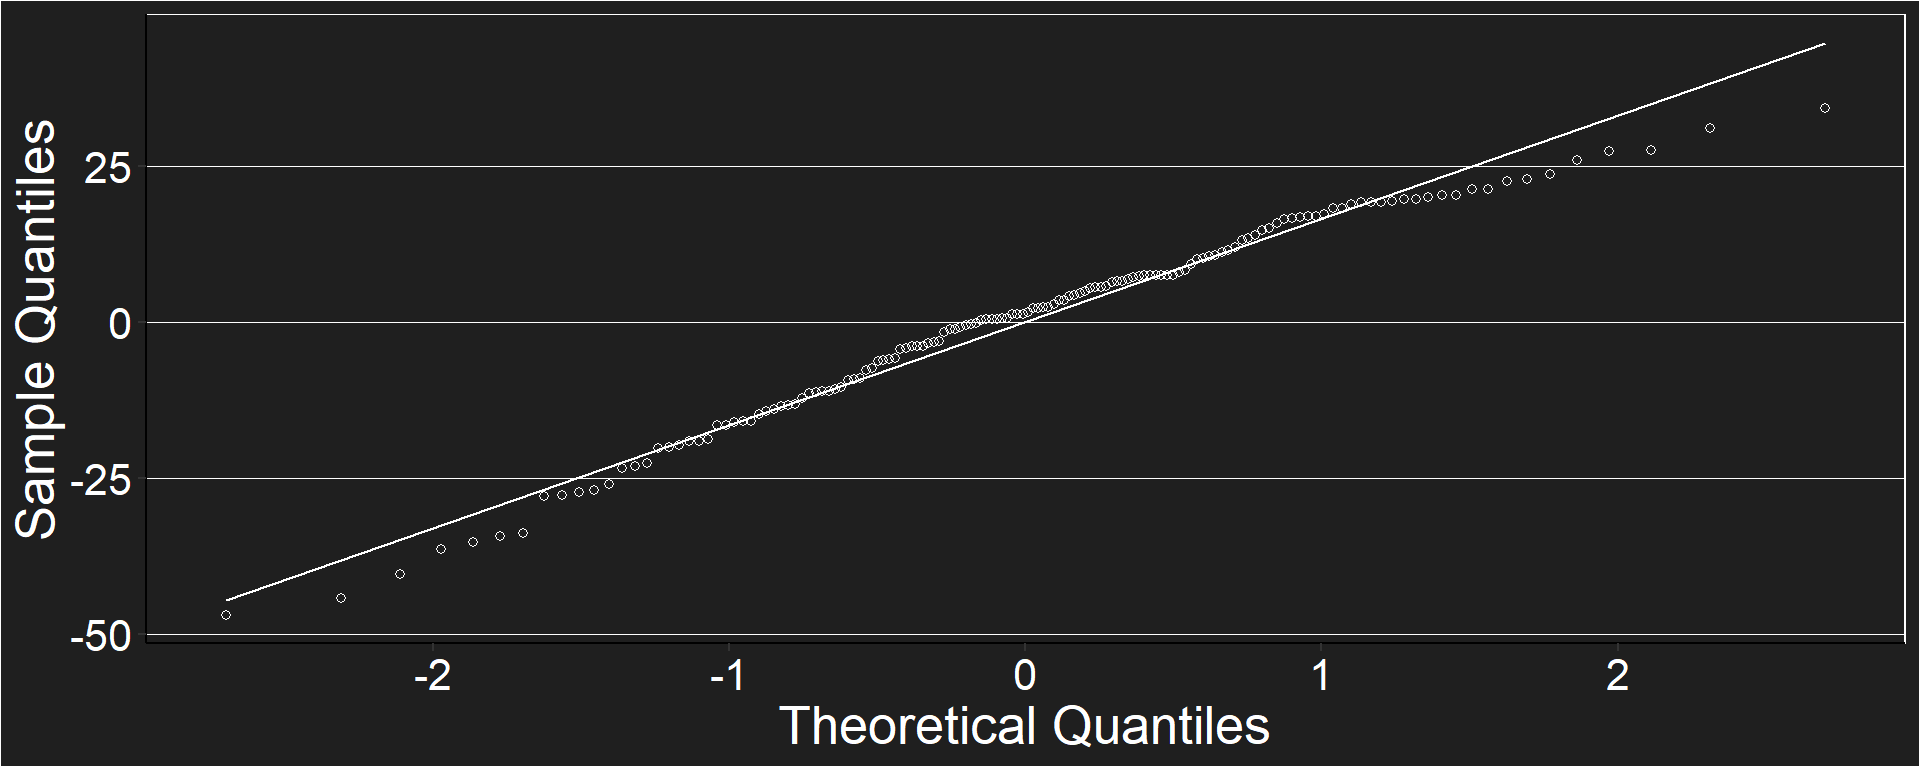
\includegraphics[width=0.95\linewidth]{madAcids_files/figure-latex/unnamed-chunk-8-2} \end{center}

\begin{verbatim}
## 
##  Shapiro-Wilk normality test
## 
## data:  e
## W = 0.9776689, p-value = 0.849326
\end{verbatim}

Anova

\begin{verbatim}
##             numDF denDF    F-value p-value
## (Intercept)     1    18 3901.69682  <.0001
## MAD             3    18    4.45443  0.0165
\end{verbatim}

Test de Tukey

\begin{verbatim}
## $emmeans
##  MAD     emmean          SE df   lower.CL   upper.CL
##  I   26.6378330 0.642202482  2 23.8746587 29.4010073
##  MM  25.3039855 0.642202482  2 22.5408112 28.0671598
##  M   25.4177998 0.642202482  2 22.6546256 28.1809741
##  SM  27.8187827 0.642202482  2 25.0556084 30.5819569
## 
## Degrees-of-freedom method: containment 
## Confidence level used: 0.95 
## 
## $contrasts
##  contrast     estimate         SE df t.ratio p.value
##  I - MM    1.333847500 0.79198912 18   1.684  0.3602
##  I - M     1.220033167 0.79198912 18   1.540  0.4354
##  I - SM   -1.180949667 0.79198912 18  -1.491  0.4629
##  MM - M   -0.113814333 0.79198912 18  -0.144  0.9989
##  MM - SM  -2.514797167 0.79198912 18  -3.175  0.0246
##  M - SM   -2.400982833 0.79198912 18  -3.032  0.0331
## 
## Degrees-of-freedom method: containment 
## P value adjustment: tukey method for comparing a family of 4 estimates
\end{verbatim}

\begin{center}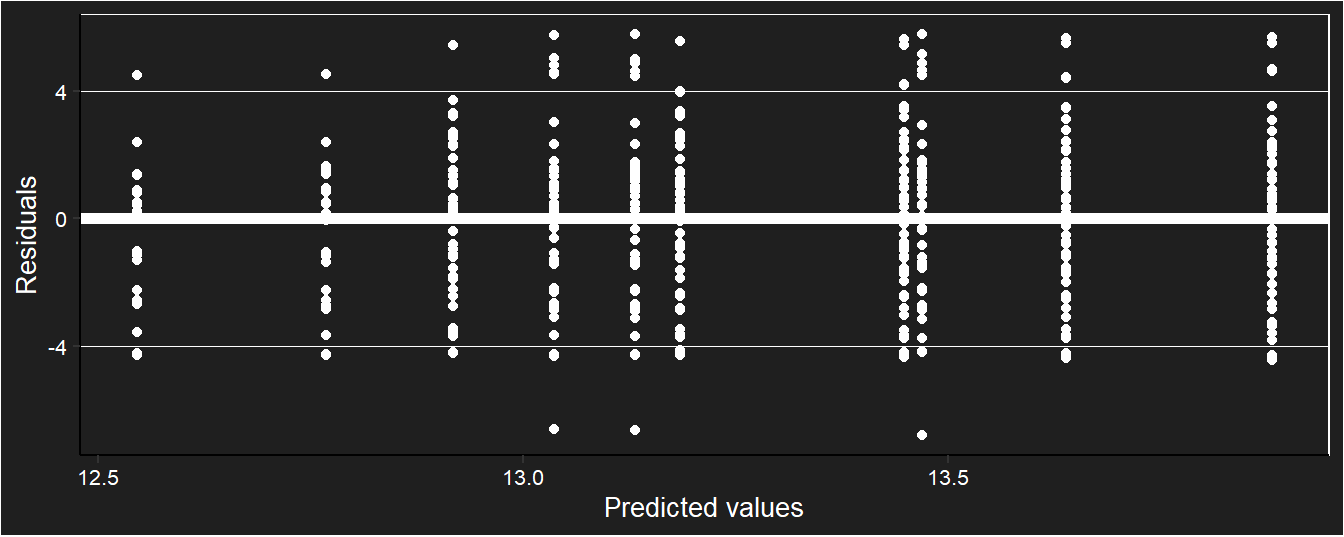
\includegraphics[width=0.95\linewidth]{madAcids_files/figure-latex/unnamed-chunk-10-1} \end{center}

\subsection{Ácido Tartárico}\label{uxe1cido-tartuxe1rico}

Modelo y supuestos

\begin{verbatim}
## Linear mixed-effects model fit by REML
##   Data: tar 
##   Log-restricted-likelihood: 39.7876038
##   Fixed: CONF ~ MAD 
##     (Intercept)           MADMM            MADM           MADSM 
## -1.16339963e-17 -1.91612264e-18  1.38777878e-17  1.15256167e-01 
## 
## Random effects:
##  Formula: ~1 | REP
##          (Intercept)     Residual
## StdDev: 0.0108045226 0.0265232023
## 
## Number of Observations: 24
## Number of Groups: 3
\end{verbatim}

\begin{center}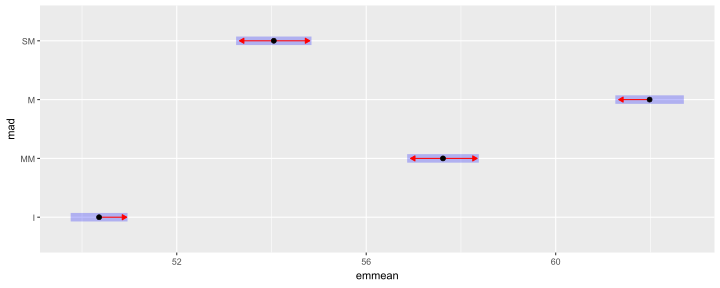
\includegraphics[width=0.95\linewidth]{madAcids_files/figure-latex/unnamed-chunk-12-1} \end{center}

\begin{center}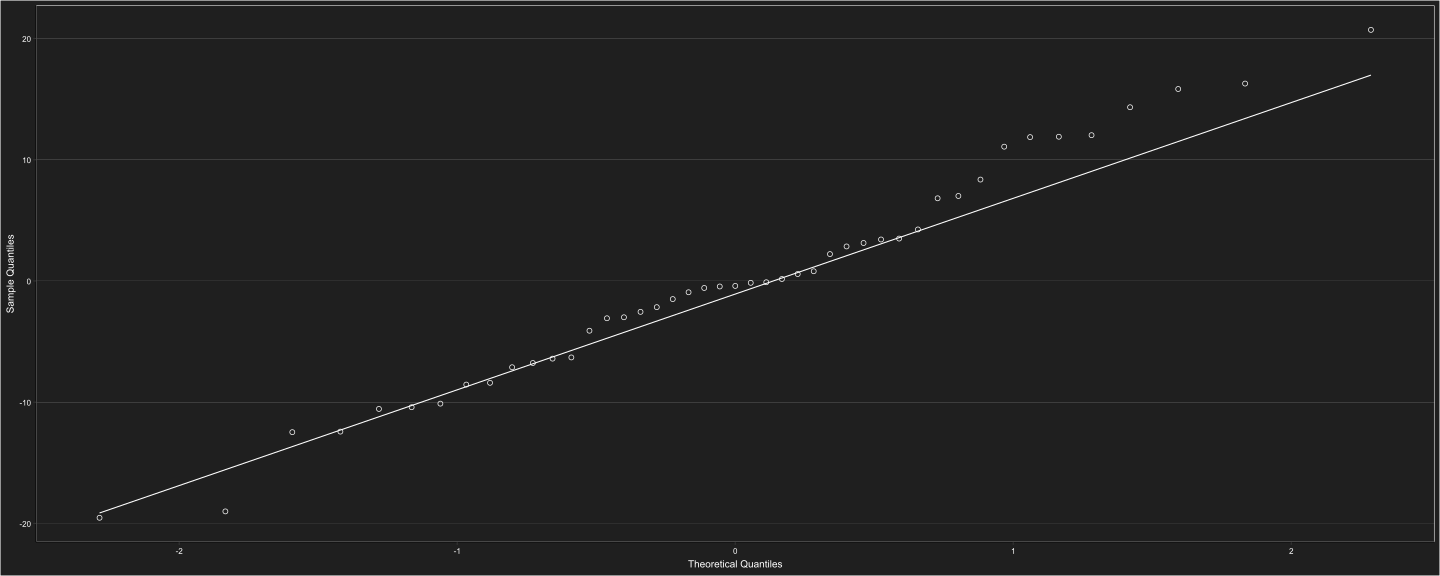
\includegraphics[width=0.95\linewidth]{madAcids_files/figure-latex/unnamed-chunk-12-2} \end{center}

\begin{verbatim}
## 
##  Shapiro-Wilk normality test
## 
## data:  e
## W = 0.7268705, p-value = 2.33095e-05
\end{verbatim}

Anova

\begin{verbatim}
##             numDF denDF    F-value p-value
## (Intercept)     1    18 12.1694124  0.0026
## MAD             3    18 28.3248543  <.0001
\end{verbatim}

Test de Tukey

\begin{verbatim}
## $emmeans
##  MAD      emmean           SE df      lower.CL     upper.CL
##  I   0.000000000 0.0124963707  2 -0.0537675433 0.0537675433
##  MM  0.000000000 0.0124963707  2 -0.0537675433 0.0537675433
##  M   0.000000000 0.0124963707  2 -0.0537675433 0.0537675433
##  SM  0.115256167 0.0124963707  2  0.0614886233 0.1690237100
## 
## Degrees-of-freedom method: containment 
## Confidence level used: 0.95 
## 
## $contrasts
##  contrast     estimate          SE df t.ratio p.value
##  I - MM    0.000000000 0.015313178 18   0.000  1.0000
##  I - M     0.000000000 0.015313178 18   0.000  1.0000
##  I - SM   -0.115256167 0.015313178 18  -7.527  <.0001
##  MM - M    0.000000000 0.015313178 18   0.000  1.0000
##  MM - SM  -0.115256167 0.015313178 18  -7.527  <.0001
##  M - SM   -0.115256167 0.015313178 18  -7.527  <.0001
## 
## Degrees-of-freedom method: containment 
## P value adjustment: tukey method for comparing a family of 4 estimates
\end{verbatim}

\begin{center}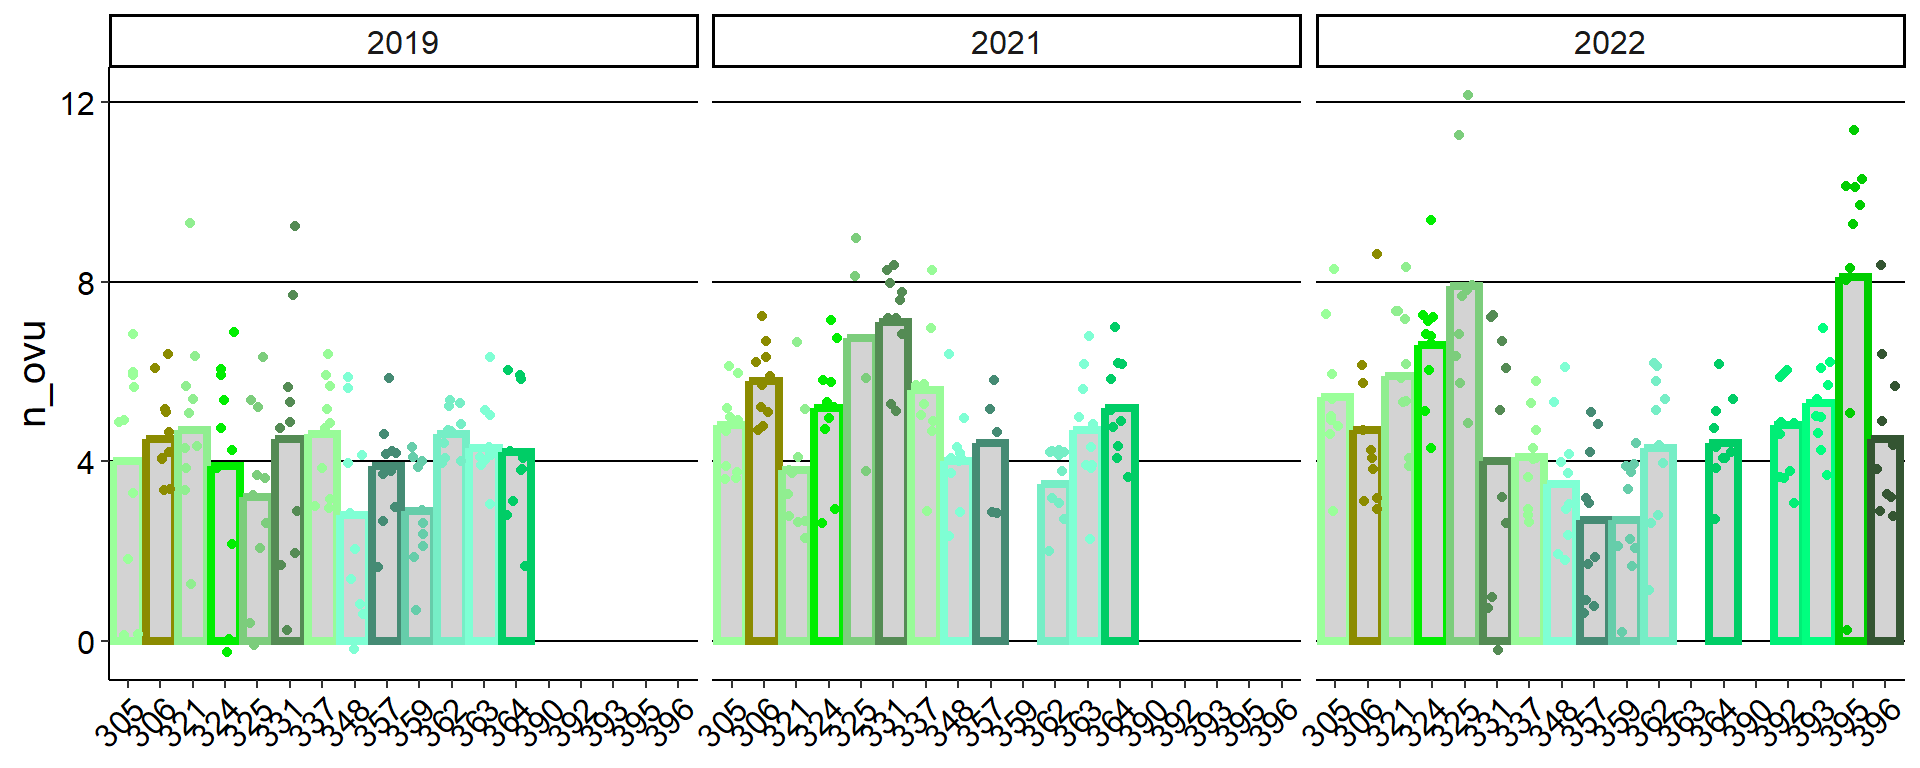
\includegraphics[width=0.95\linewidth]{madAcids_files/figure-latex/unnamed-chunk-14-1} \end{center}

\subsection{Ácido málico}\label{uxe1cido-muxe1lico}

Modelo y supuestos

\begin{verbatim}
## Linear mixed-effects model fit by REML
##   Data: mal 
##   Log-restricted-likelihood: -26.5820545
##   Fixed: CONF ~ MAD 
## (Intercept)       MADMM        MADM       MADSM 
##  7.38748867  3.58805750  4.37205000  3.14937817 
## 
## Random effects:
##  Formula: ~1 | REP
##         (Intercept)   Residual
## StdDev: 0.365216528 2.68012348
## 
## Variance function:
##  Structure: Different standard deviations per stratum
##  Formula: ~1 | MAD 
##  Parameter estimates:
##            I            M           MM           SM 
## 1.0000000000 0.0552668662 0.2702105687 0.2600800859 
## Number of Observations: 24
## Number of Groups: 3
\end{verbatim}

\begin{center}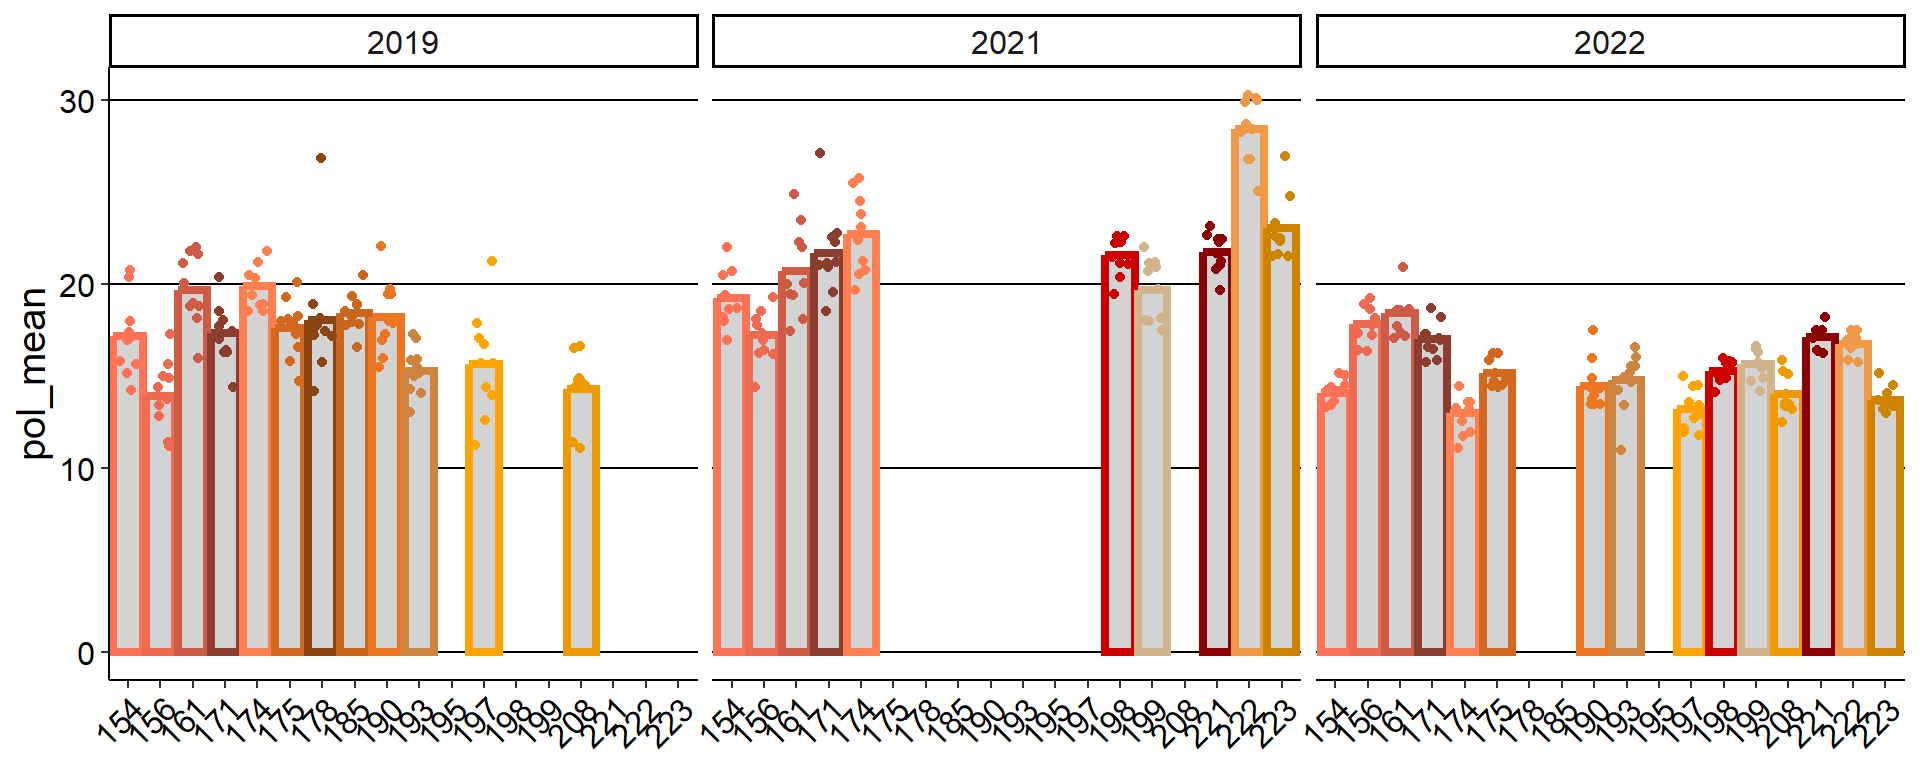
\includegraphics[width=0.95\linewidth]{madAcids_files/figure-latex/unnamed-chunk-16-1} \end{center}

\begin{center}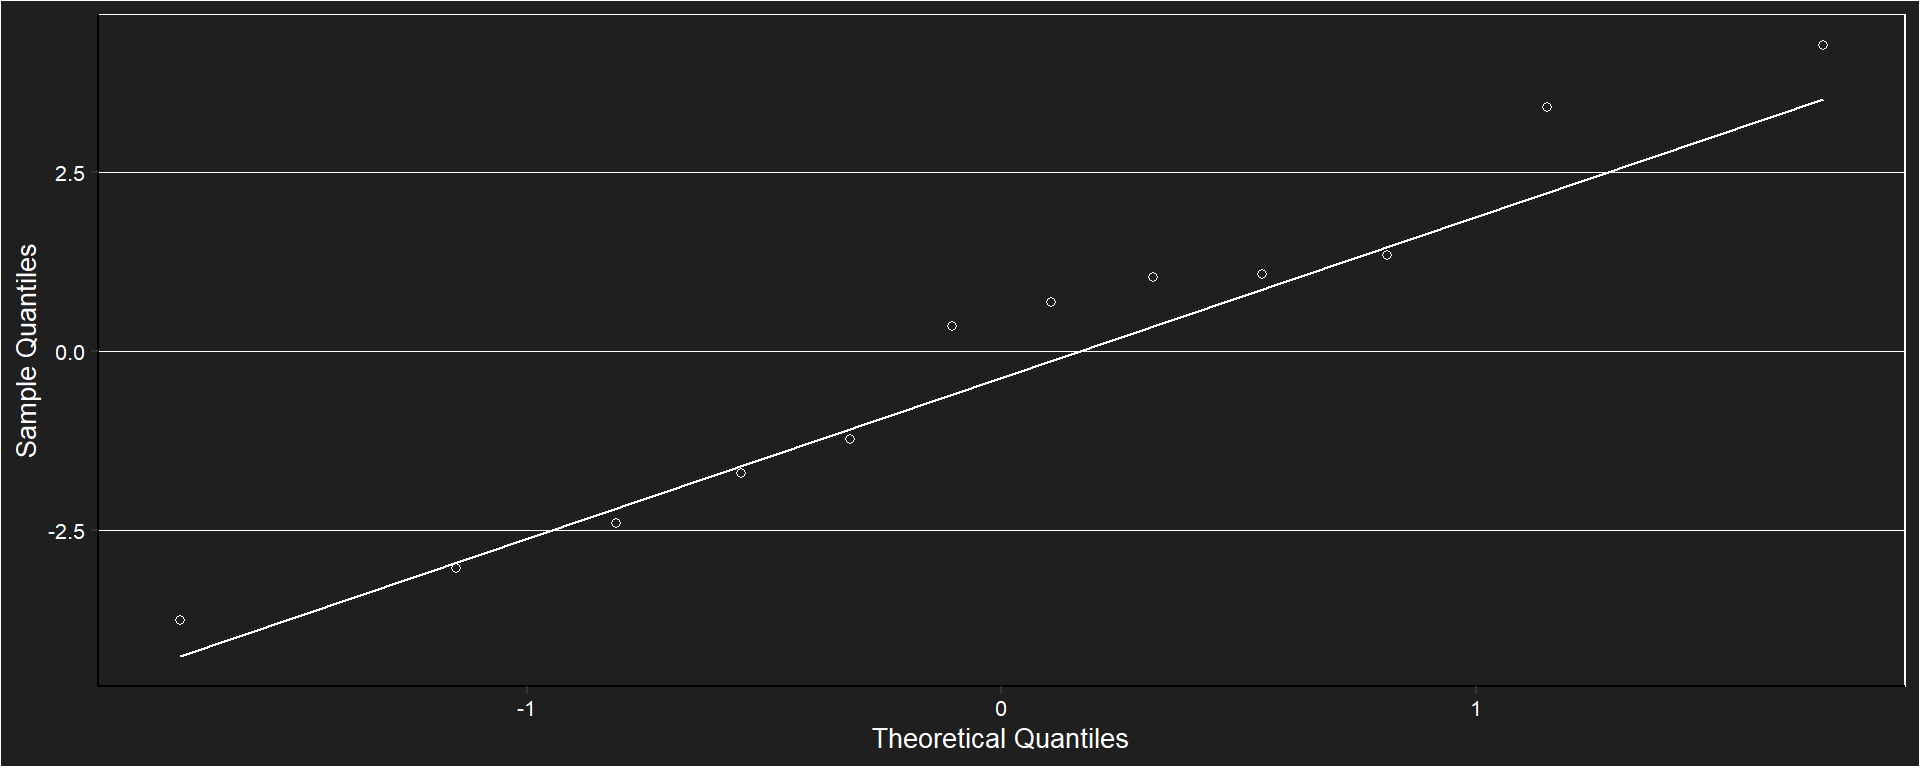
\includegraphics[width=0.95\linewidth]{madAcids_files/figure-latex/unnamed-chunk-16-2} \end{center}

\begin{verbatim}
## 
##  Shapiro-Wilk normality test
## 
## data:  e
## W = 0.8897338, p-value = 0.0131242
\end{verbatim}

Anova

\begin{verbatim}
##             numDF denDF     F-value p-value
## (Intercept)     1    18 2846.522875  <.0001
## MAD             3    18   12.960439   1e-04
\end{verbatim}

Test de Tukey

\begin{verbatim}
## $emmeans
##  MAD      emmean          SE df    lower.CL   upper.CL
##  I    7.38748867 1.114288120  2  2.59309384 12.1818835
##  MM  10.97554617 0.363141046  2  9.41307635 12.5380160
##  M   11.75953867 0.219357531  2 10.81571939 12.7033579
##  SM  10.53686683 0.354175189  2  9.01297399 12.0607597
## 
## Degrees-of-freedom method: containment 
## Confidence level used: 0.95 
## 
## $contrasts
##  contrast    estimate          SE df t.ratio p.value
##  I - MM   -3.58805750 1.133396383 18  -3.166  0.0251
##  I - M    -4.37205000 1.095825564 18  -3.990  0.0043
##  I - SM   -3.14937817 1.130555618 18  -2.786  0.0542
##  MM - M   -0.78399250 0.301773212 18  -2.598  0.0780
##  MM - SM   0.43867933 0.410352787 18   1.069  0.7121
##  M - SM    1.22267183 0.290922183 18   4.203  0.0027
## 
## Degrees-of-freedom method: containment 
## P value adjustment: tukey method for comparing a family of 4 estimates
\end{verbatim}

\begin{center}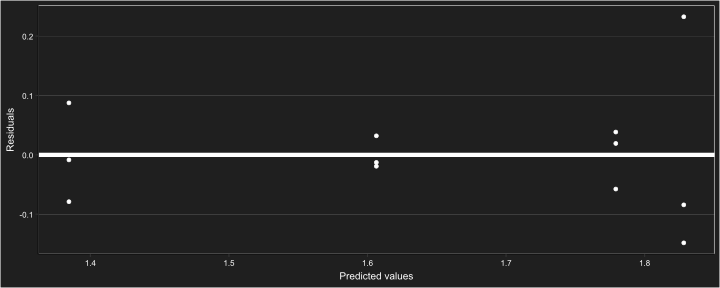
\includegraphics[width=0.95\linewidth]{madAcids_files/figure-latex/unnamed-chunk-18-1} \end{center}

\subsection{Ácido quínico}\label{uxe1cido-quuxednico}

Modelo y supuestos

\begin{verbatim}
## Linear mixed-effects model fit by REML
##   Data: qui 
##   Log-restricted-likelihood: -11.8097603
##   Fixed: CONF ~ MAD 
##  (Intercept)        MADMM         MADM        MADSM 
## 0.0665693333 3.0094548333 2.4789668333 2.7825800000 
## 
## Random effects:
##  Formula: ~1 | REP
##         (Intercept)   Residual
## StdDev: 0.180571585 0.34446664
## 
## Number of Observations: 24
## Number of Groups: 3
\end{verbatim}

\begin{center}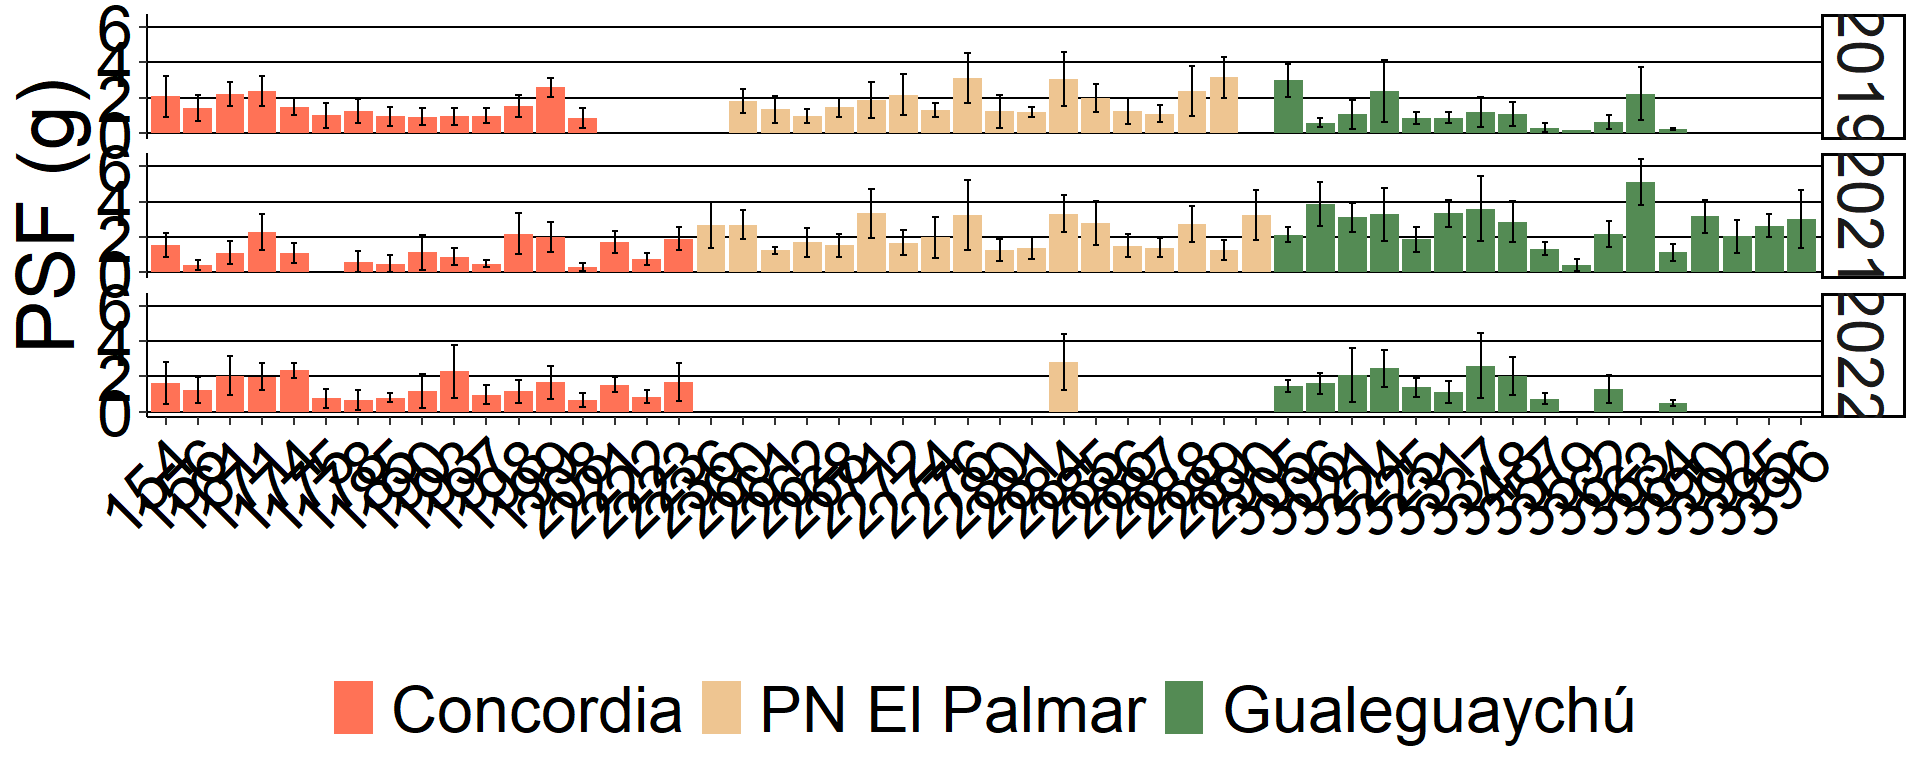
\includegraphics[width=0.95\linewidth]{madAcids_files/figure-latex/unnamed-chunk-21-1} \end{center}

\begin{center}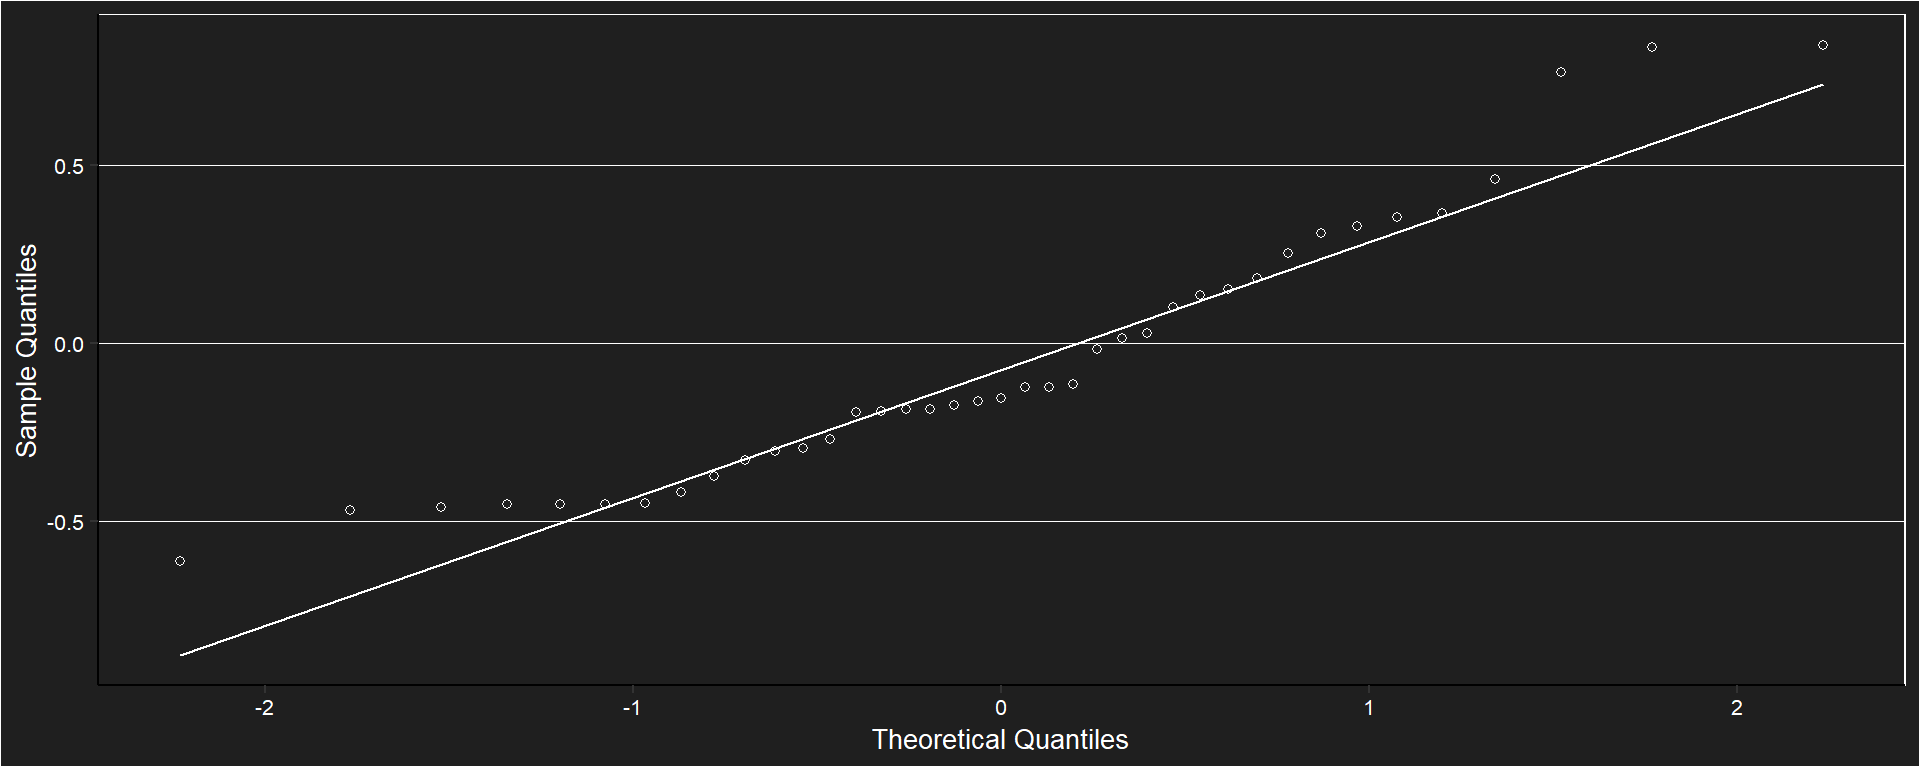
\includegraphics[width=0.95\linewidth]{madAcids_files/figure-latex/unnamed-chunk-21-2} \end{center}

\begin{verbatim}
## 
##  Shapiro-Wilk normality test
## 
## data:  e
## W = 0.9324113, p-value = 0.110376
\end{verbatim}

\begin{verbatim}
## Levene's Test for Homogeneity of Variance (center = median)
##       Df F value   Pr(>F)  
## group  3 3.05613 0.052027 .
##       20                   
## ---
## Signif. codes:  0 '***' 0.001 '**' 0.01 '*' 0.05 '.' 0.1 ' ' 1
\end{verbatim}

Anova

\begin{verbatim}
##             numDF denDF     F-value p-value
## (Intercept)     1    18 288.0789394  <.0001
## MAD             3    18  98.4765528  <.0001
\end{verbatim}

Test de Tukey

\begin{verbatim}
## $emmeans
##  MAD      emmean          SE df     lower.CL   upper.CL
##  I   0.066569333 0.175056877  2 -0.686639616 0.81977828
##  MM  3.076024167 0.175056877  2  2.322815217 3.82923312
##  M   2.545536167 0.175056877  2  1.792327217 3.29874512
##  SM  2.849149333 0.175056877  2  2.095940384 3.60235828
## 
## Degrees-of-freedom method: containment 
## Confidence level used: 0.95 
## 
## $contrasts
##  contrast     estimate          SE df t.ratio p.value
##  I - MM   -3.009454833 0.198877907 18 -15.132  <.0001
##  I - M    -2.478966833 0.198877907 18 -12.465  <.0001
##  I - SM   -2.782580000 0.198877907 18 -13.991  <.0001
##  MM - M    0.530488000 0.198877907 18   2.667  0.0683
##  MM - SM   0.226874833 0.198877907 18   1.141  0.6700
##  M - SM   -0.303613167 0.198877907 18  -1.527  0.4431
## 
## Degrees-of-freedom method: containment 
## P value adjustment: tukey method for comparing a family of 4 estimates
\end{verbatim}

\begin{center}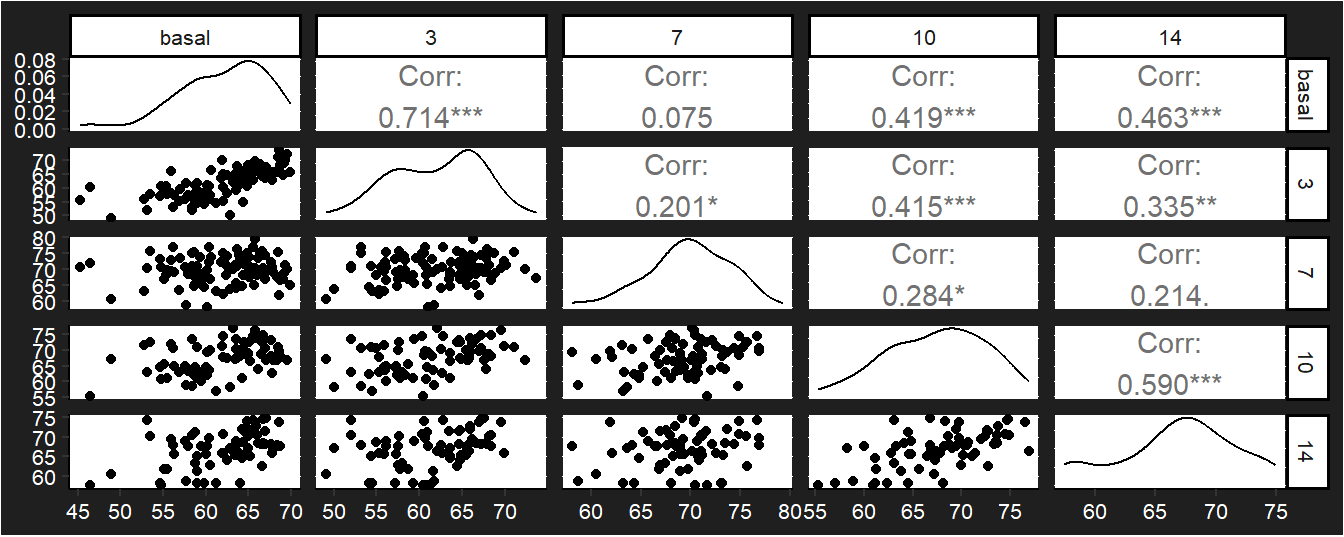
\includegraphics[width=0.95\linewidth]{madAcids_files/figure-latex/unnamed-chunk-23-1} \end{center}

\subsection{Ácido succinico}\label{uxe1cido-succinico}

Modelo y supuestos

\begin{center}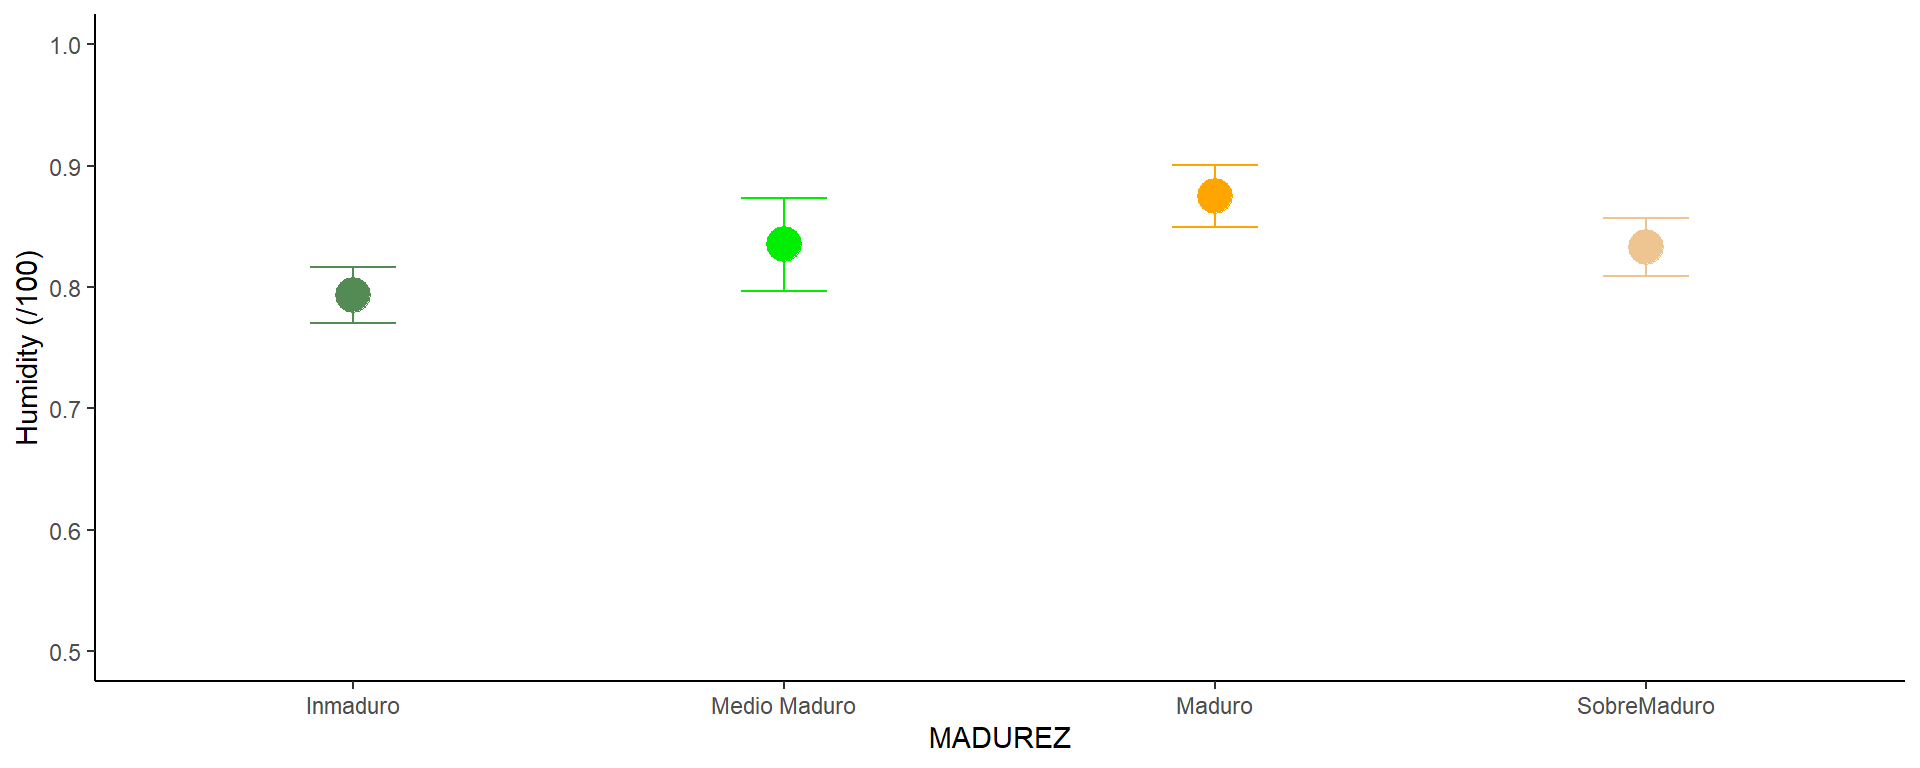
\includegraphics[width=0.95\linewidth]{madAcids_files/figure-latex/unnamed-chunk-24-1} \end{center}

\begin{center}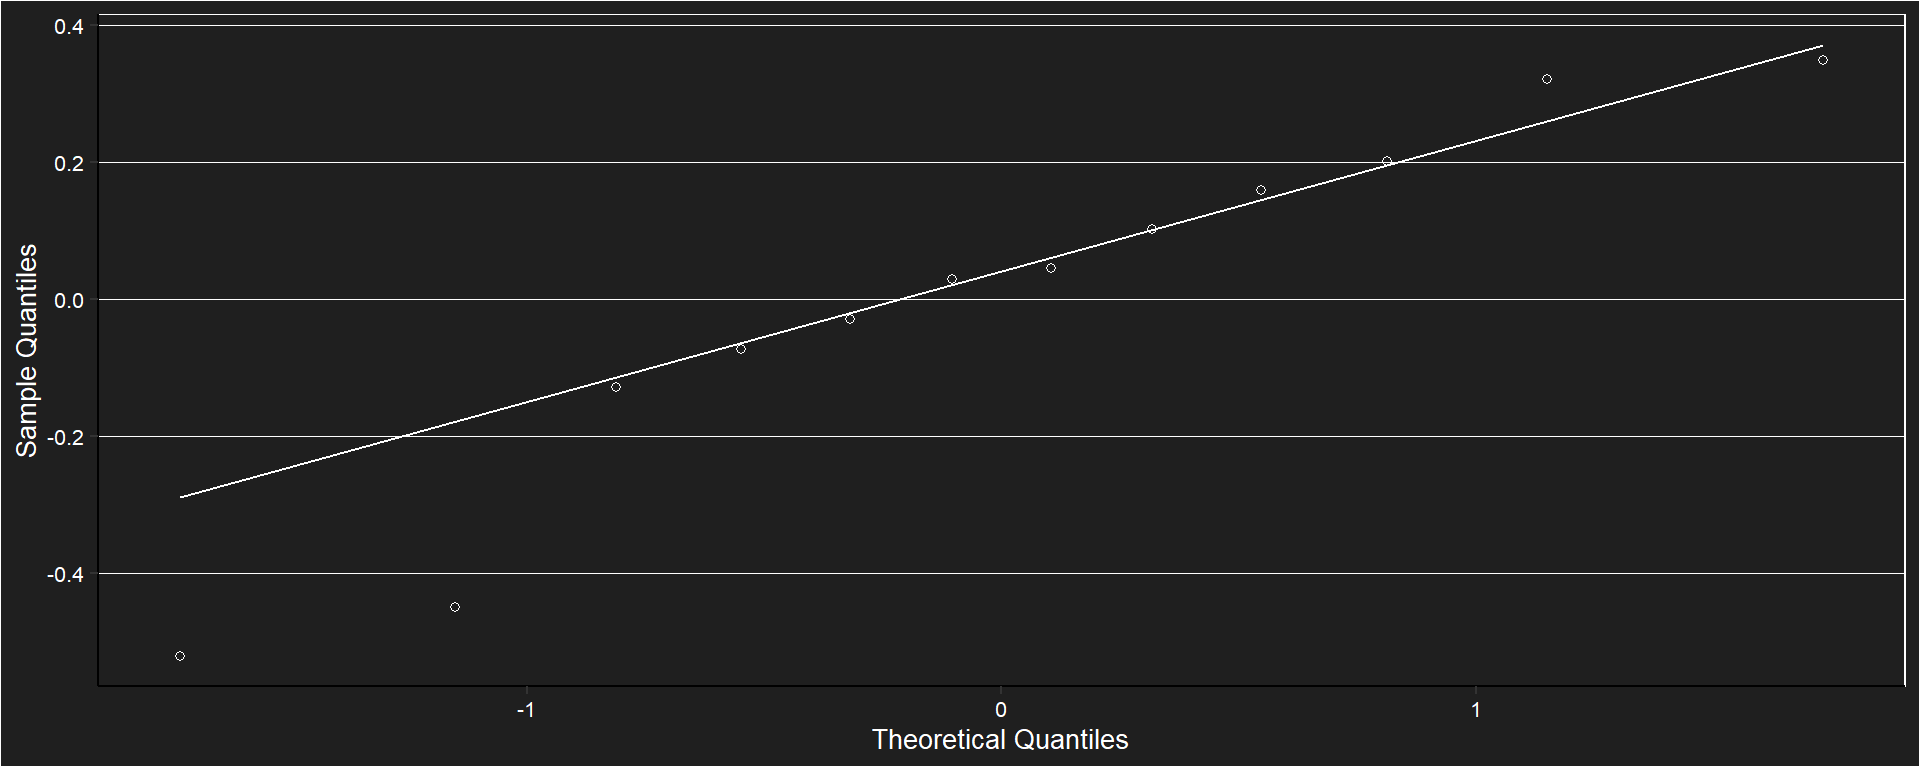
\includegraphics[width=0.95\linewidth]{madAcids_files/figure-latex/unnamed-chunk-24-2} \end{center}

\begin{verbatim}
## 
##  Shapiro-Wilk normality test
## 
## data:  e
## W = 0.8253994, p-value = 0.000789836
\end{verbatim}

\begin{verbatim}
## Levene's Test for Homogeneity of Variance (center = median)
##       Df F value Pr(>F)
## group  3 1.89009 0.1638
##       20
\end{verbatim}

Anova

\begin{verbatim}
##             numDF denDF    F-value p-value
## (Intercept)     1    18 667.582635  <.0001
## MAD             3    18  97.574430  <.0001
\end{verbatim}

Test de Tukey

\begin{verbatim}
## $emmeans
##  MAD     emmean          SE df    lower.CL   upper.CL
##  I   19.1837748 0.634030365  2 16.45576235 21.9117873
##  MM  11.2524155 0.634030365  2  8.52440302 13.9804280
##  M   11.1127248 0.634030365  2  8.38471235 13.8407373
##  SM  14.3175103 0.634030365  2 11.58949785 17.0455228
## 
## Degrees-of-freedom method: containment 
## Confidence level used: 0.95 
## 
## $contrasts
##  contrast    estimate          SE df t.ratio p.value
##  I - MM    7.93135933 0.541102157 18  14.658  <.0001
##  I - M     8.07105000 0.541102157 18  14.916  <.0001
##  I - SM    4.86626450 0.541102157 18   8.993  <.0001
##  MM - M    0.13969067 0.541102157 18   0.258  0.9938
##  MM - SM  -3.06509483 0.541102157 18  -5.665  0.0001
##  M - SM   -3.20478550 0.541102157 18  -5.923  0.0001
## 
## Degrees-of-freedom method: containment 
## P value adjustment: tukey method for comparing a family of 4 estimates
\end{verbatim}

\begin{center}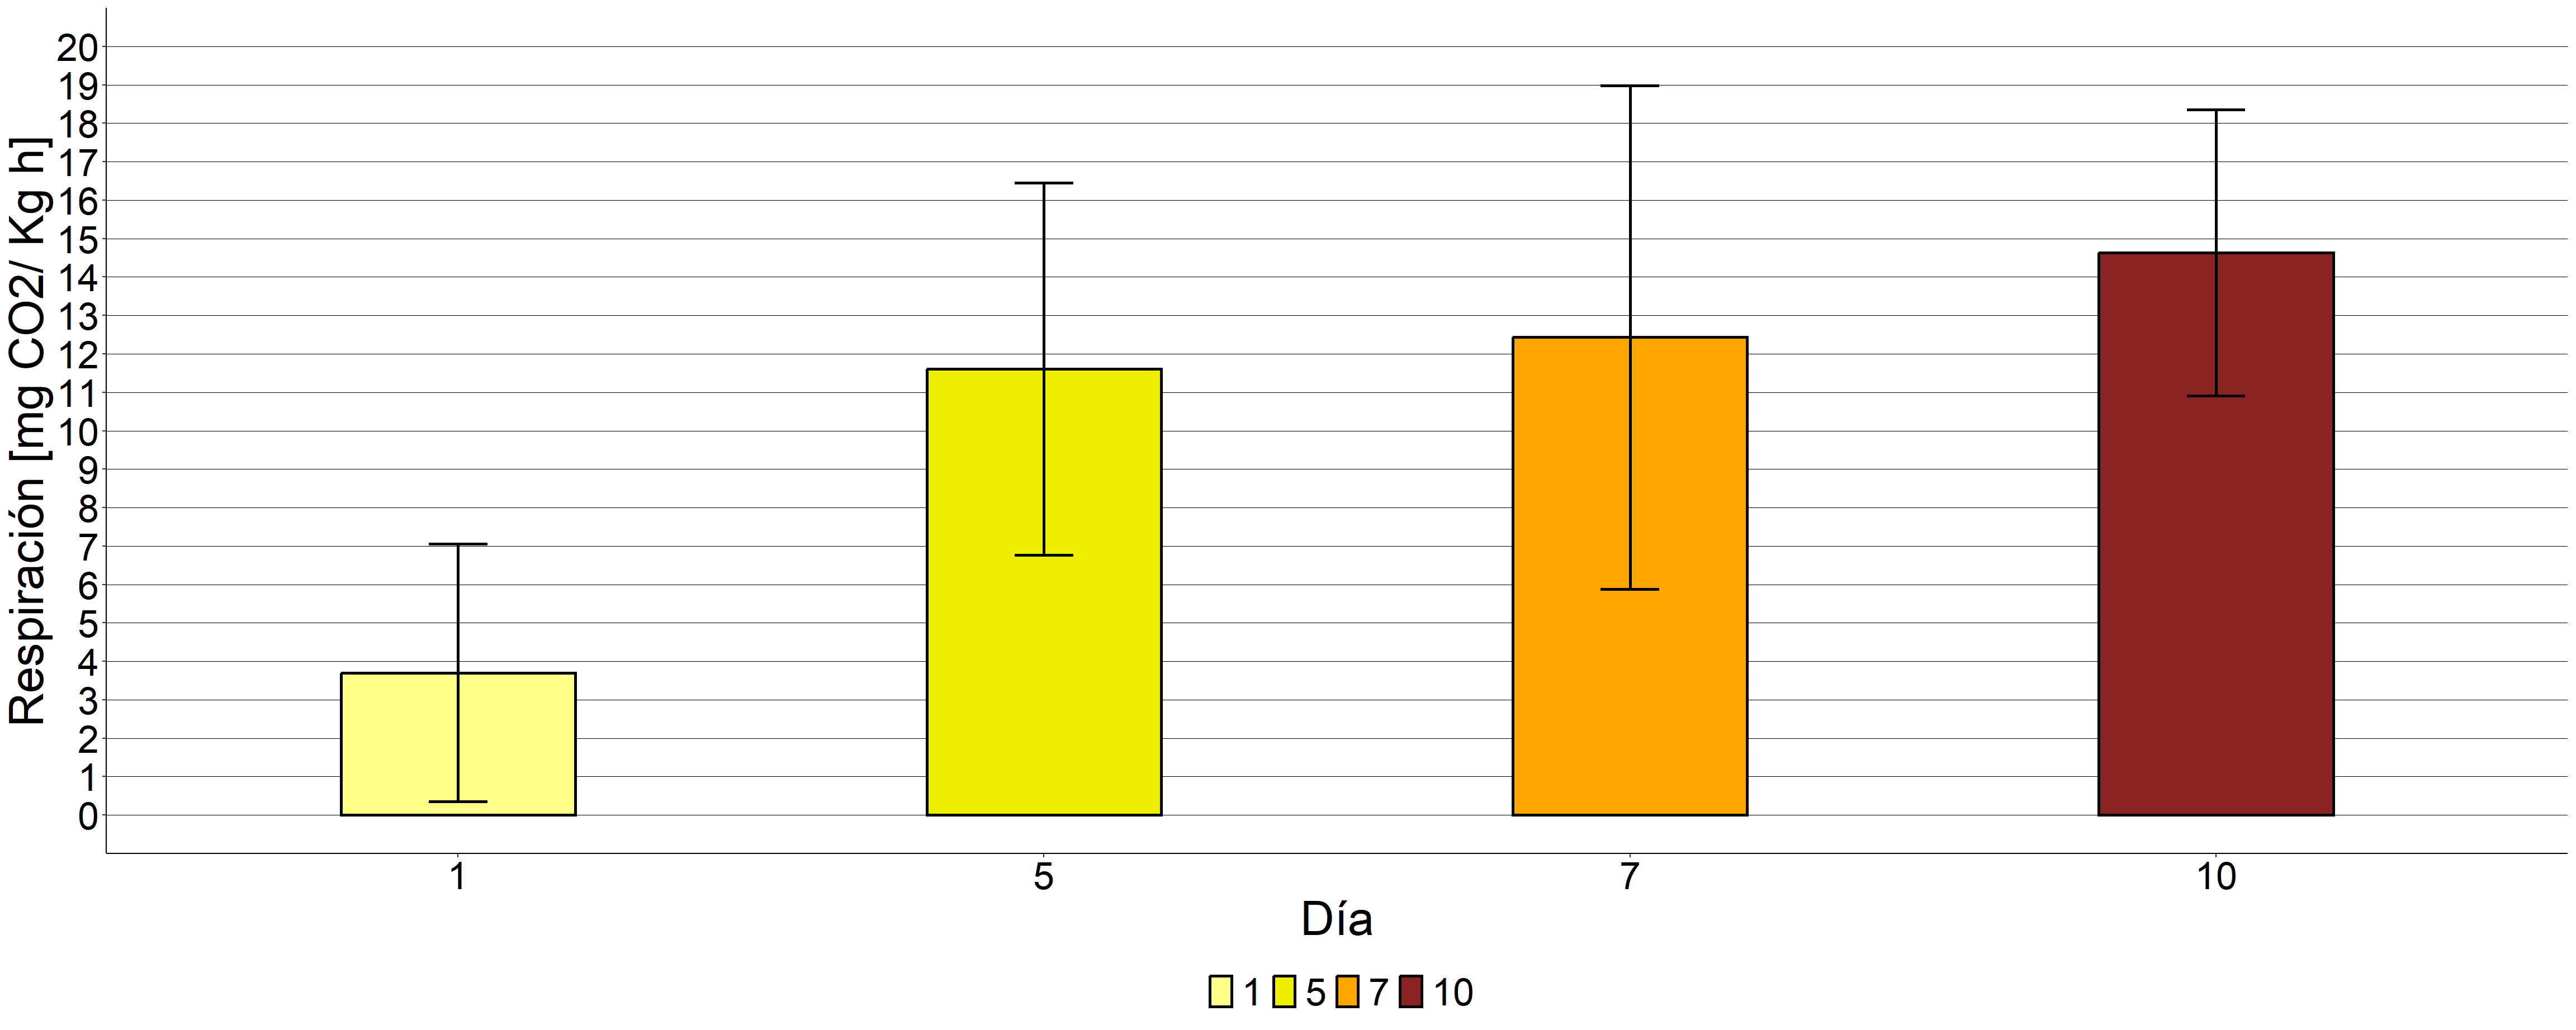
\includegraphics[width=0.95\linewidth]{madAcids_files/figure-latex/unnamed-chunk-26-1} \end{center}

\section{Acidos orgánicos en peso
seco}\label{acidos-orguxe1nicos-en-peso-seco}

Concentración del perfíl de ácidos orgánicos

\begin{center}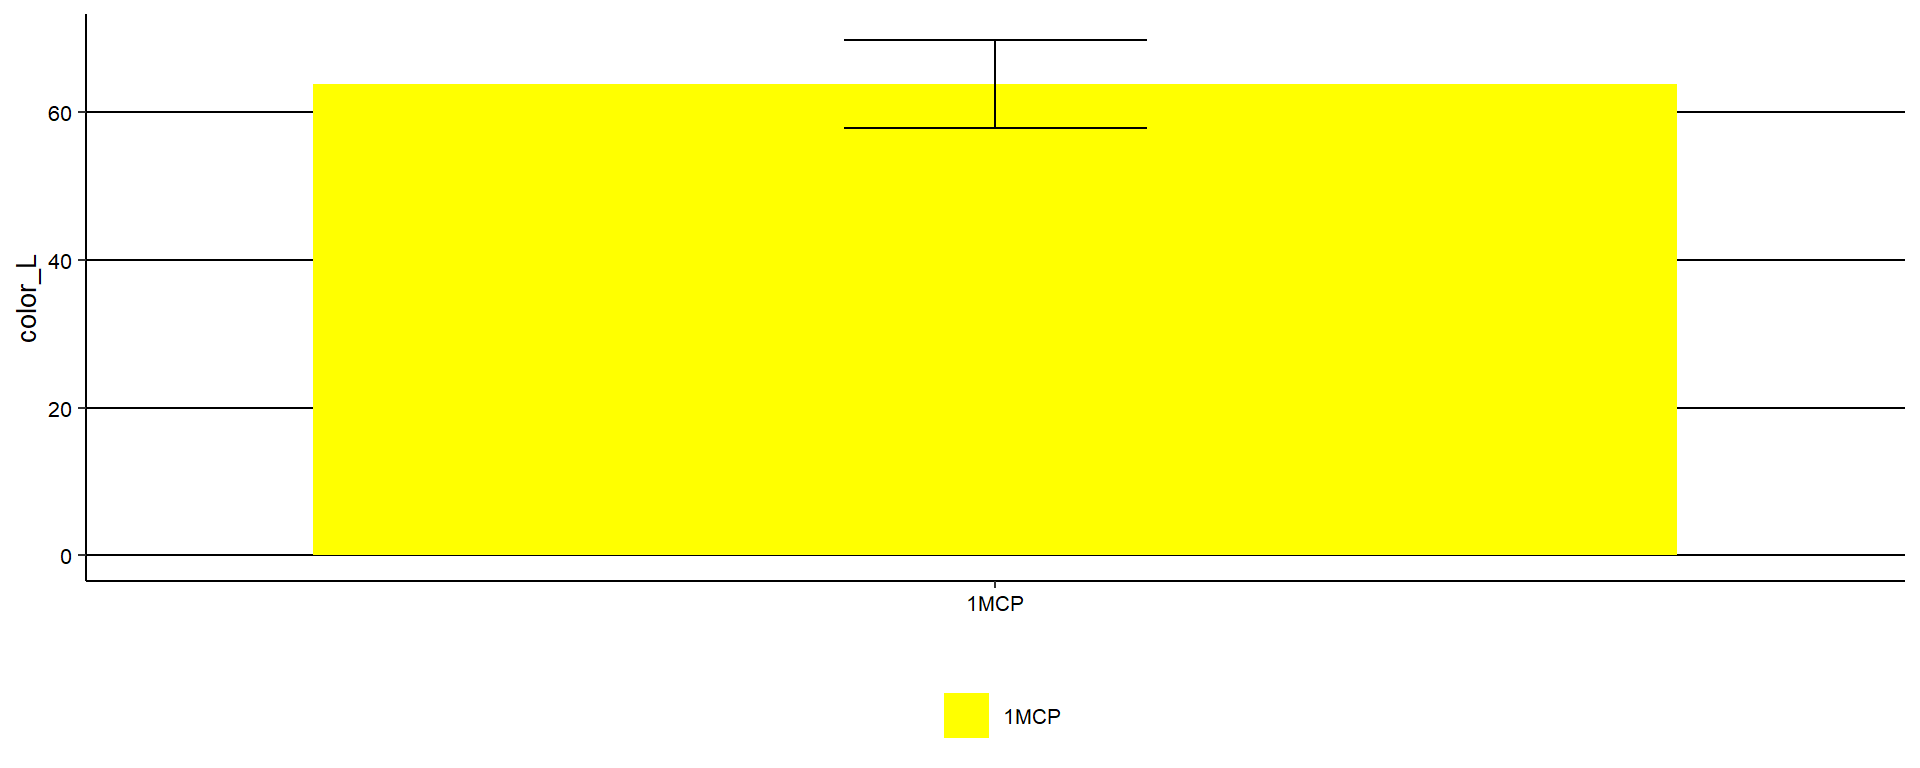
\includegraphics[width=0.95\linewidth]{madAcids_files/figure-latex/unnamed-chunk-27-1} \end{center}

Tabla descriptiva

\begin{verbatim}
##          CAR MAD N          CONS            sd            se            ci
## 1  Tartárico   I 6   0.000000000  0.0000000000  0.0000000000  0.0000000000
## 2  Tartárico  MM 6   0.000000000  0.0000000000  0.0000000000  0.0000000000
## 3  Tartárico   M 6   0.000000000  0.0000000000  0.0000000000  0.0000000000
## 4  Tartárico  SM 6   0.941135667  0.4830674796  0.1972114727  0.5069482296
## 5     Málico   I 6  44.902134000 19.1523848051  7.8189283550 20.0991952034
## 6     Málico  MM 6  90.189531667  4.0220151138  1.6419807944  4.2208460046
## 7     Málico   M 6 105.147489667  3.3635751544  1.3731738066  3.5298556445
## 8     Málico  SM 6  84.794599167  5.3680332445  2.1914903952  5.6334054030
## 9    Quínico   I 6   0.440663333  0.6826727005  0.2786999629  0.7164210623
## 10   Quínico  MM 6  25.317606333  3.8140013880  1.5570595465  4.0025489871
## 11   Quínico   M 6  22.688808167  2.2426216210  0.9155464429  2.3534870559
## 12   Quínico  SM 6  22.920424500  3.7568053163  1.5337093480  3.9425253911
## 13 Succínico   I 6 112.333486500  6.5345265736  2.6677093027  6.8575650762
## 14 Succínico  MM 6  92.481592333  4.7805090422  1.9516346440  5.0168365657
## 15 Succínico   M 6  99.437239833  4.8240138759  1.9693954180  5.0624920887
## 16 Succínico  SM 6 115.655151333 12.4187930831  5.0699510458 13.0327240659
## 17       ATT   I 3   1.779200000  0.0507984252  0.0293284844  0.1261902837
## 18       ATT  MM 3   1.606400000  0.0278969532  0.0161063135  0.0692998736
## 19       ATT   M 3   1.828266667  0.2039063837  0.1177254055  0.5065315375
## 20       ATT  SM 3   1.384533333  0.0835275603  0.0482246594  0.2074939626
## 21   TOTALac   I 6 157.676283833 24.4147956495  9.9672985859 25.6217566954
## 22   TOTALac  MM 6 207.988730333 11.6569574255  4.7589329410 12.2332265750
## 23   TOTALac   M 6 227.273537667  4.2846255274  1.7491910468  4.4964387320
## 24   TOTALac  SM 6 224.311310667 13.9874059778  5.7103345784 14.6788823428
## 25      <NA>   I 6 266.880791667  8.4819431471  3.4627387896  8.9012534341
## 26      <NA>  MM 6 301.680354667 34.6167224669 14.1322177686 36.3280222931
## 27      <NA>   M 6 350.625756167 31.1823867560 12.7301560857 32.7239079987
## 28      <NA>  SM 6 428.368083167 26.7527791069 10.9217763355 28.0753198610
\end{verbatim}

Evolución del perfíl de ácidos orgánicos

\begin{verbatim}
## Error in `palette()`:
## ! Insufficient values in manual scale. 6 needed but only 4 provided.
\end{verbatim}

\subsection{Ácidos orgánicos
totales}\label{uxe1cidos-orguxe1nicos-totales}

\begin{center}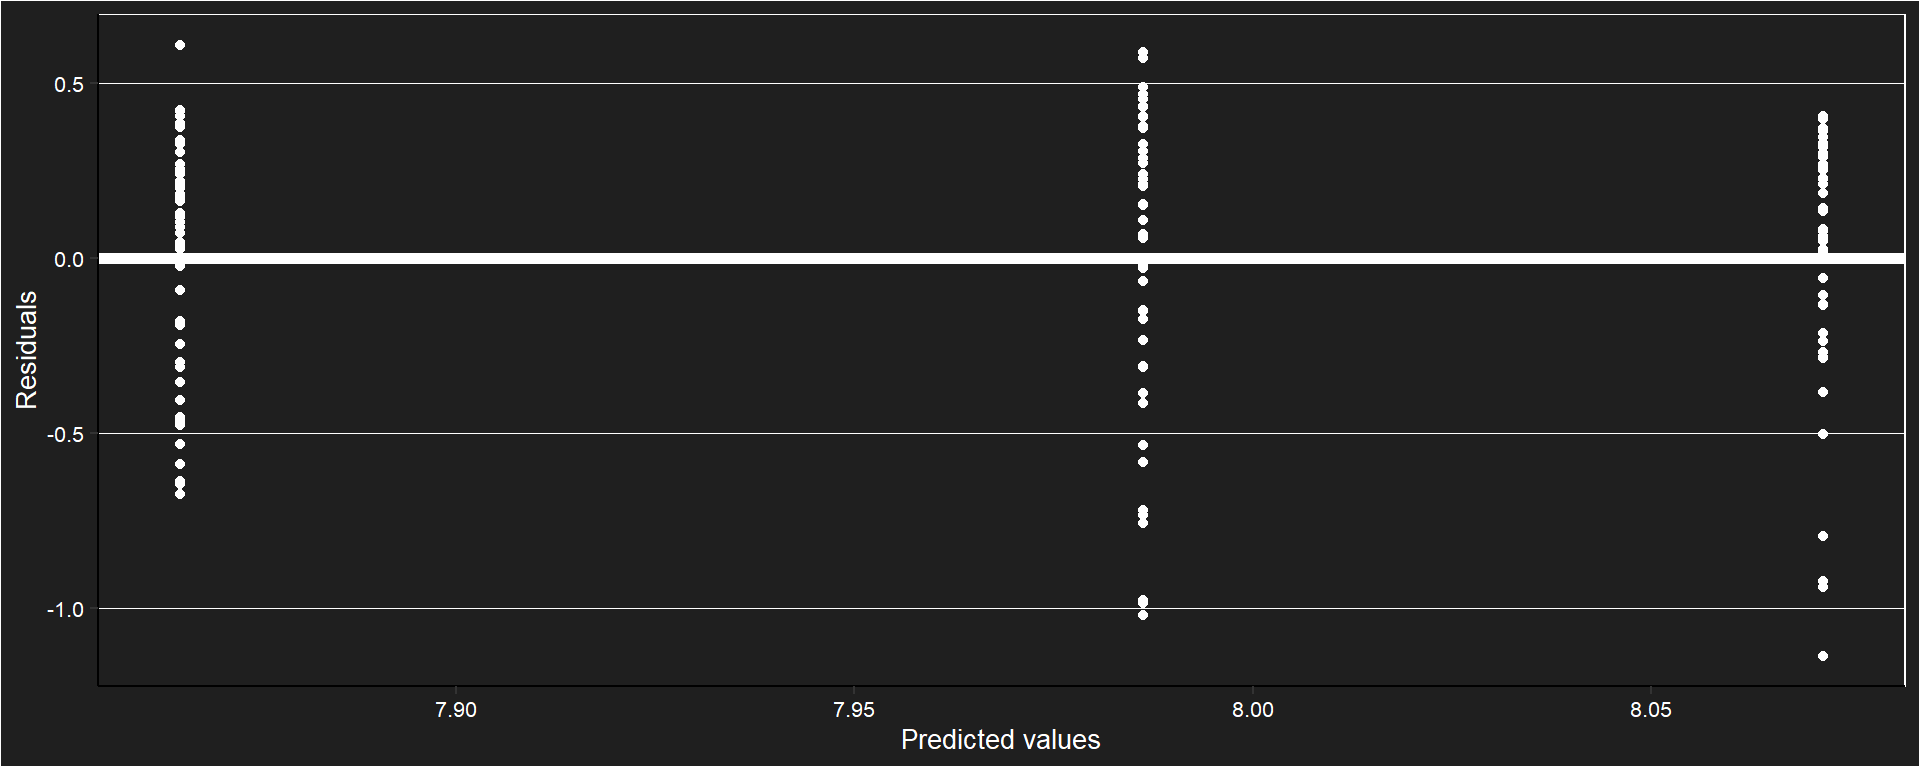
\includegraphics[width=0.95\linewidth]{madAcids_files/figure-latex/unnamed-chunk-30-1} \end{center}

Tabla descriptiva totales

\begin{verbatim}
##        CAR MAD N       TOTALS             sd             se            ci
## 1    ACIDS   I 6 157.67628383 24.41479564951  9.96729858594 25.6217566954
## 2    ACIDS  MM 6 207.98873017 11.65695733461  4.75893290386 12.2332264797
## 3    ACIDS   M 6 227.27353783  4.28462560986  1.74919108050  4.4964388186
## 4    ACIDS  SM 6 224.31131067 13.98740580960  5.71033450979 14.6788821663
## 5  CATIONS   I 3  20.97175533  7.74194818235  4.46981586713 19.2320654422
## 6  CATIONS  MM 3  21.05341000  2.57785325998  1.48832427358  6.4037424985
## 7  CATIONS   M 3  23.27046433  2.76151278503  1.59436014981  6.8599780508
## 8  CATIONS  SM 3  17.82636733  3.17591985185  1.83361818139  7.8894222735
## 9     STAT   I 3   1.72112247  0.26333177284  0.15203466994  0.6541523876
## 10    STAT  MM 3   1.44765169  0.11629091852  0.06714059311  0.2888826562
## 11    STAT   M 3   1.54171591  0.13269129972  0.07660935761  0.3296234617
## 12    STAT  SM 3   1.90950427  0.00773336868  0.00446486249  0.0192107528
## 13  SUGARS   I 6 266.88079200  8.48194327733  3.46273884278  8.9012535708
## 14  SUGARS  MM 6 301.68035450 34.61672214508 14.13221763719 36.3280219554
## 15  SUGARS   M 6 350.62575617 31.18238675596 12.73015608570 32.7239079987
## 16  SUGARS  SM 6 428.36808300 26.75277856794 10.92177611552 28.0753192954
\end{verbatim}

Modelo y supuestos

\begin{verbatim}
## Linear mixed-effects model fit by REML
##   Data: dataAT 
##   Log-restricted-likelihood: -86.6219141
##   Fixed: TOTALS ~ MAD 
## (Intercept)       MADMM        MADM       MADSM 
## 157.6762838  50.3124463  69.5972540  66.6350268 
## 
## Random effects:
##  Formula: ~1 | REP
##         (Intercept)   Residual
## StdDev:  0.11875108 15.3782993
## 
## Number of Observations: 24
## Number of Groups: 3
\end{verbatim}

\begin{center}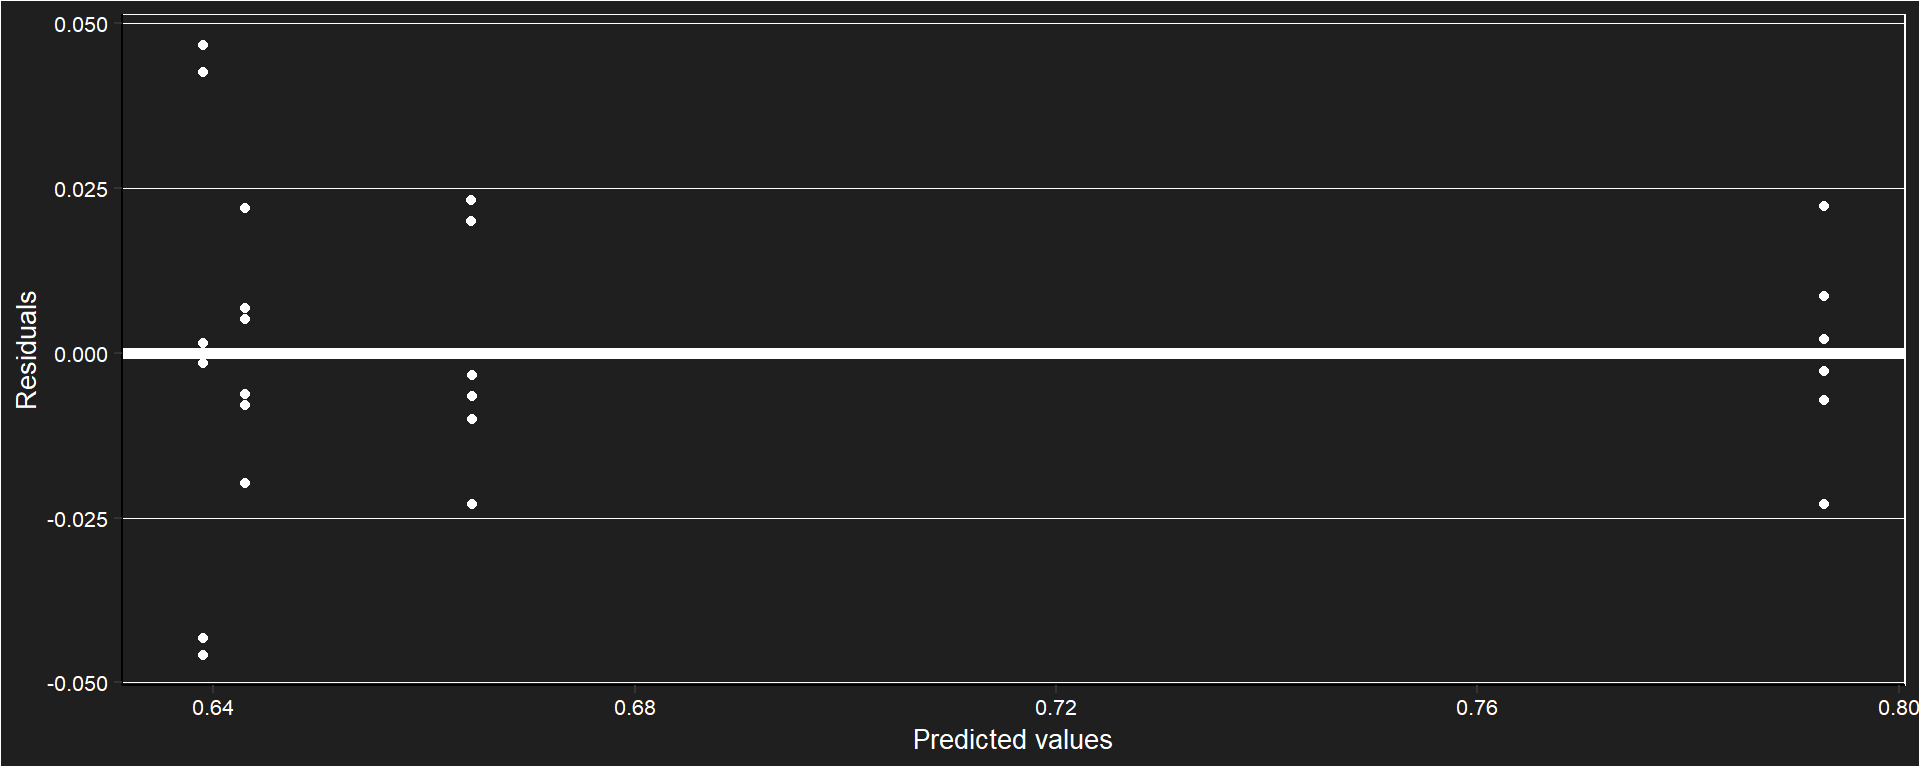
\includegraphics[width=0.95\linewidth]{madAcids_files/figure-latex/unnamed-chunk-32-1} \end{center}

\begin{center}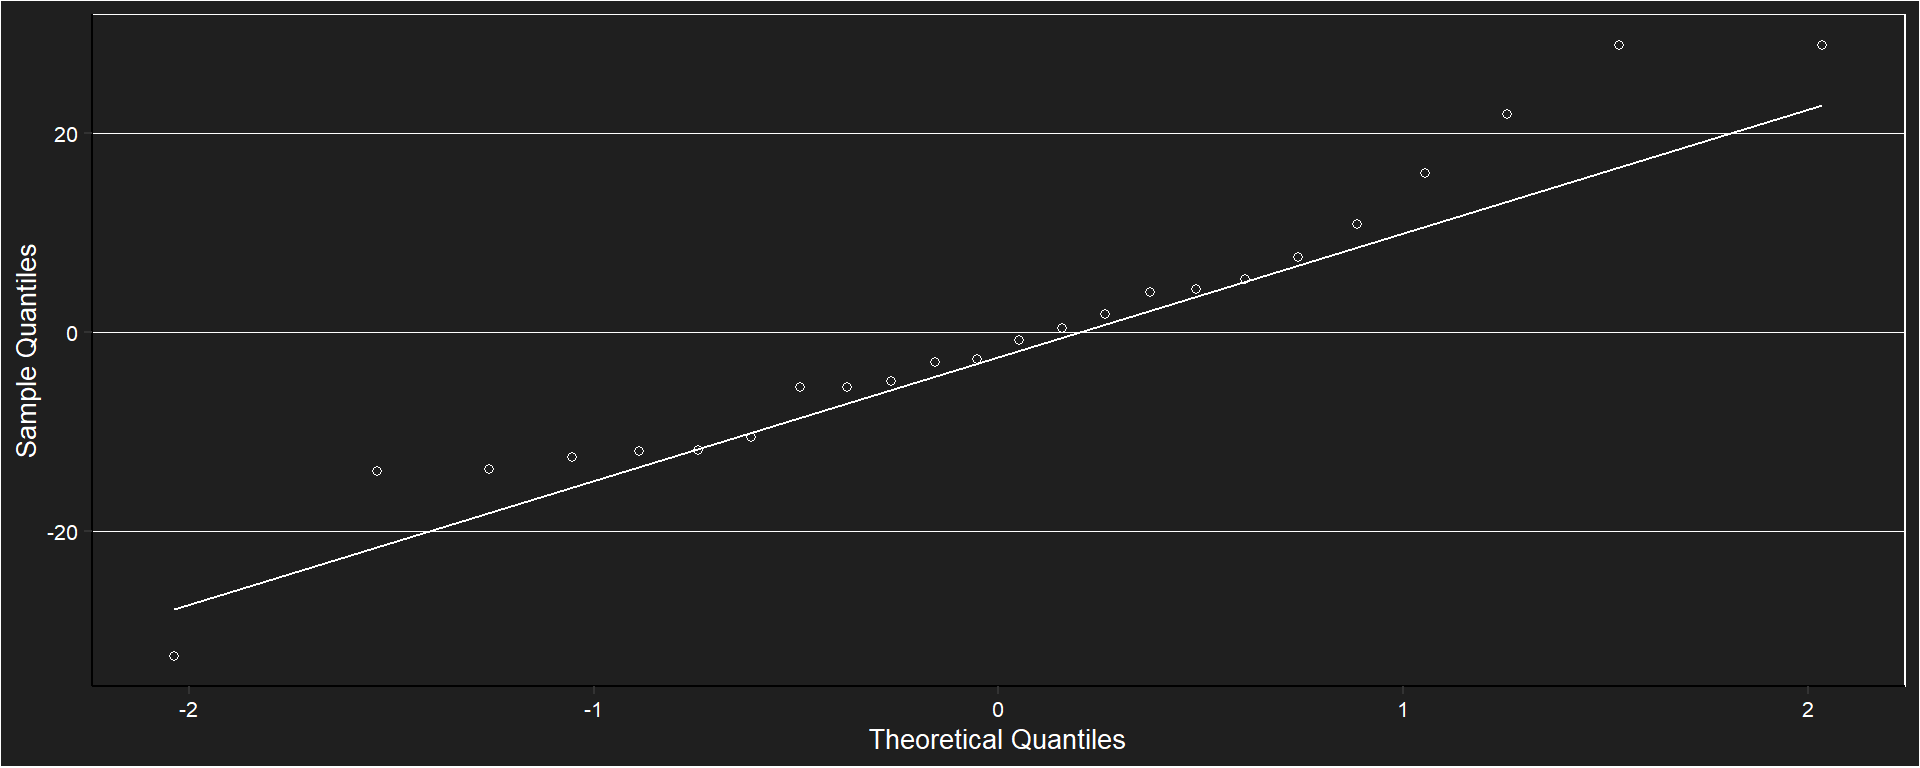
\includegraphics[width=0.95\linewidth]{madAcids_files/figure-latex/unnamed-chunk-32-2} \end{center}

\begin{verbatim}
## 
##  Shapiro-Wilk normality test
## 
## data:  e
## W = 0.9558794, p-value = 0.361338
\end{verbatim}

Anova

\begin{verbatim}
##             numDF denDF    F-value p-value
## (Intercept)     1    18 4234.25715  <.0001
## MAD             3    18   26.34856  <.0001
\end{verbatim}

Test de Tukey

\begin{verbatim}
## $emmeans
##  MAD     emmean         SE df   lower.CL   upper.CL
##  I   157.676284 6.27853875  2 130.661912 184.690656
##  MM  207.988730 6.27853875  2 180.974358 235.003102
##  M   227.273538 6.27853875  2 200.259166 254.287910
##  SM  224.311311 6.27853875  2 197.296939 251.325683
## 
## Degrees-of-freedom method: containment 
## Confidence level used: 0.95 
## 
## $contrasts
##  contrast    estimate         SE df t.ratio p.value
##  I - MM   -50.3124463 8.87866525 18  -5.667  0.0001
##  I - M    -69.5972540 8.87866525 18  -7.839  <.0001
##  I - SM   -66.6350268 8.87866525 18  -7.505  <.0001
##  MM - M   -19.2848077 8.87866525 18  -2.172  0.1689
##  MM - SM  -16.3225805 8.87866525 18  -1.838  0.2886
##  M - SM     2.9622272 8.87866525 18   0.334  0.9868
## 
## Degrees-of-freedom method: containment 
## P value adjustment: tukey method for comparing a family of 4 estimates
\end{verbatim}

\begin{center}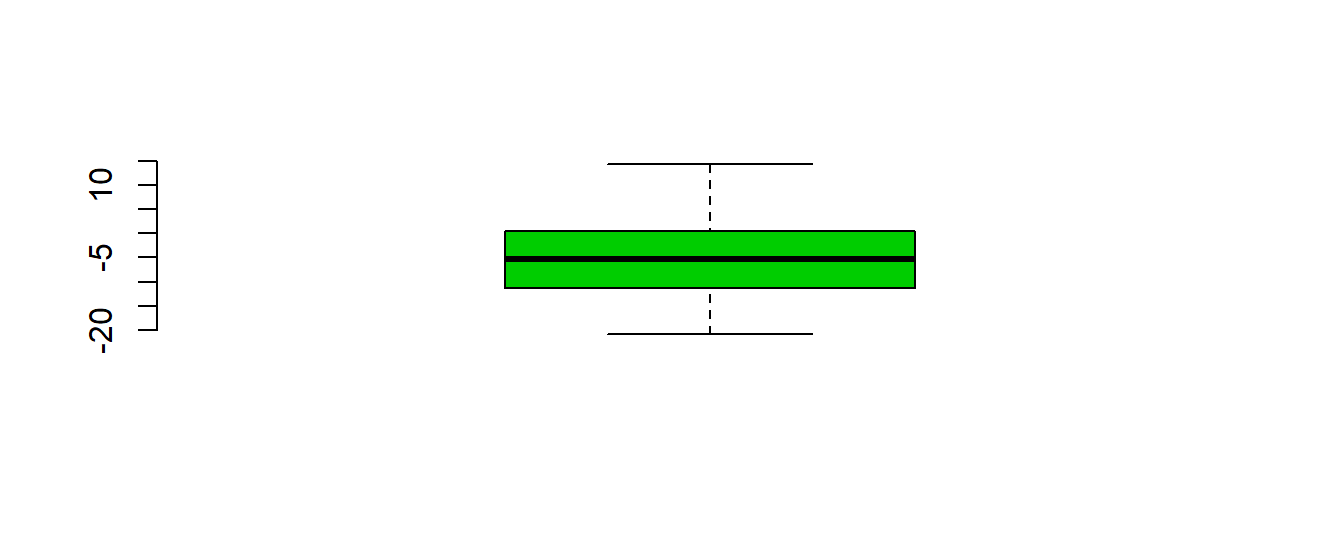
\includegraphics[width=0.95\linewidth]{madAcids_files/figure-latex/unnamed-chunk-34-1} \end{center}

Ácido tartárico

Modelo y supuestos

\begin{verbatim}
## Linear mixed-effects model fit by REML
##   Data: tar 
##   Log-restricted-likelihood: -3.09688774
##   Fixed: CONS ~ MAD 
##     (Intercept)           MADMM            MADM           MADSM 
##  8.70989721e-17 -1.26351284e-16 -2.22044605e-16  9.41135667e-01 
## 
## Random effects:
##  Formula: ~1 | REP
##         (Intercept)    Residual
## StdDev:  0.09563016 0.225881487
## 
## Number of Observations: 24
## Number of Groups: 3
\end{verbatim}

\begin{center}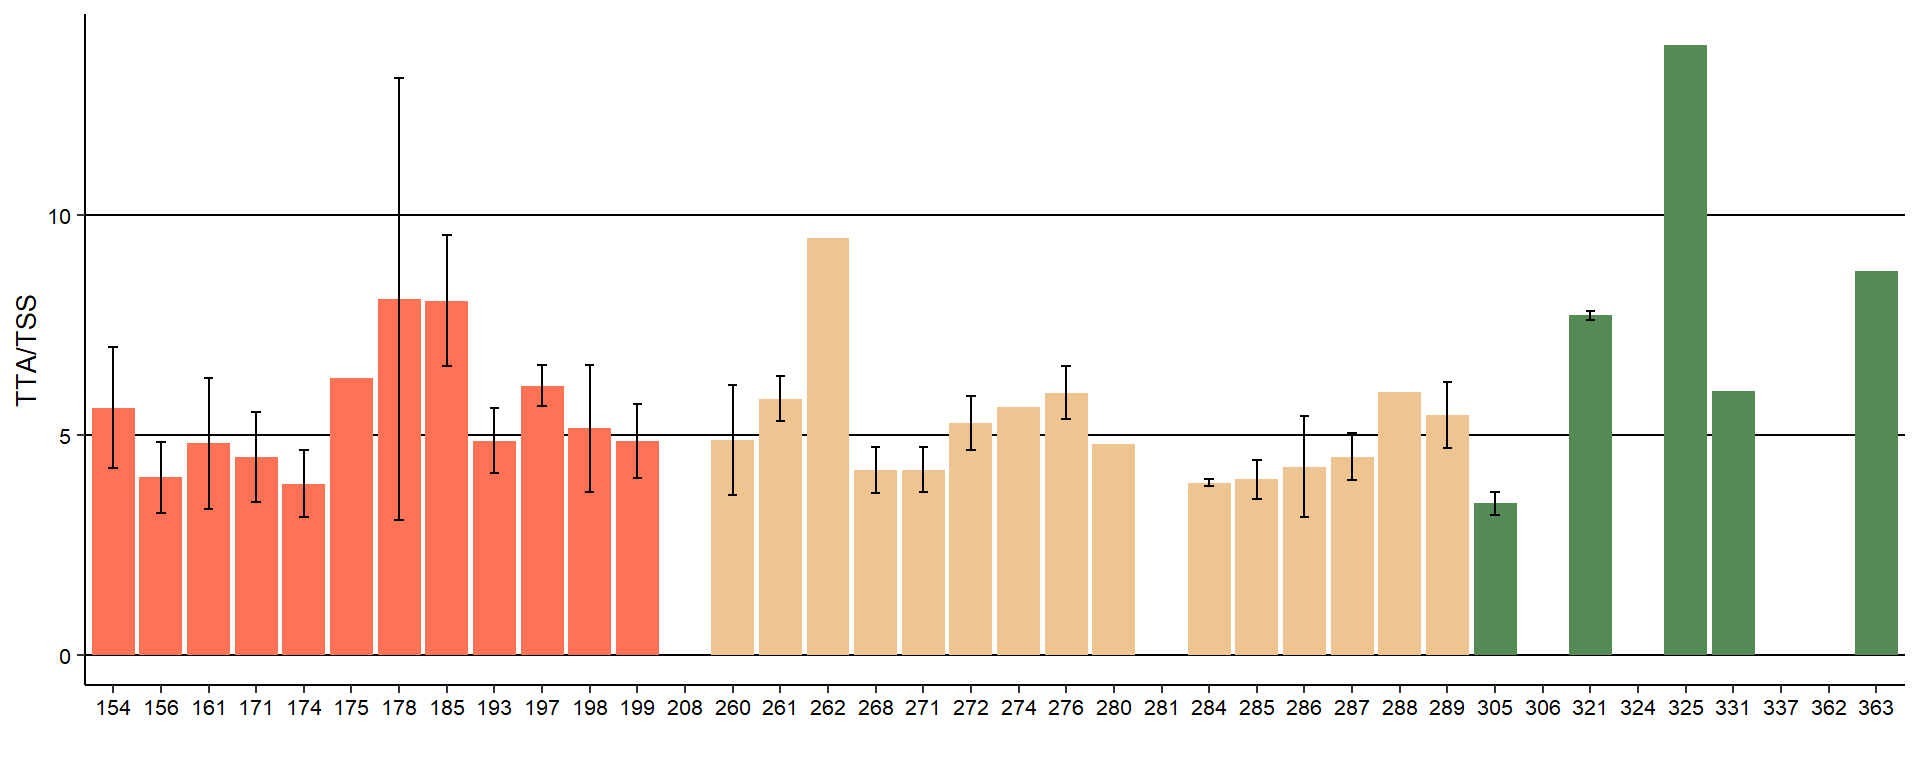
\includegraphics[width=0.95\linewidth]{madAcids_files/figure-latex/unnamed-chunk-36-1} \end{center}

\begin{center}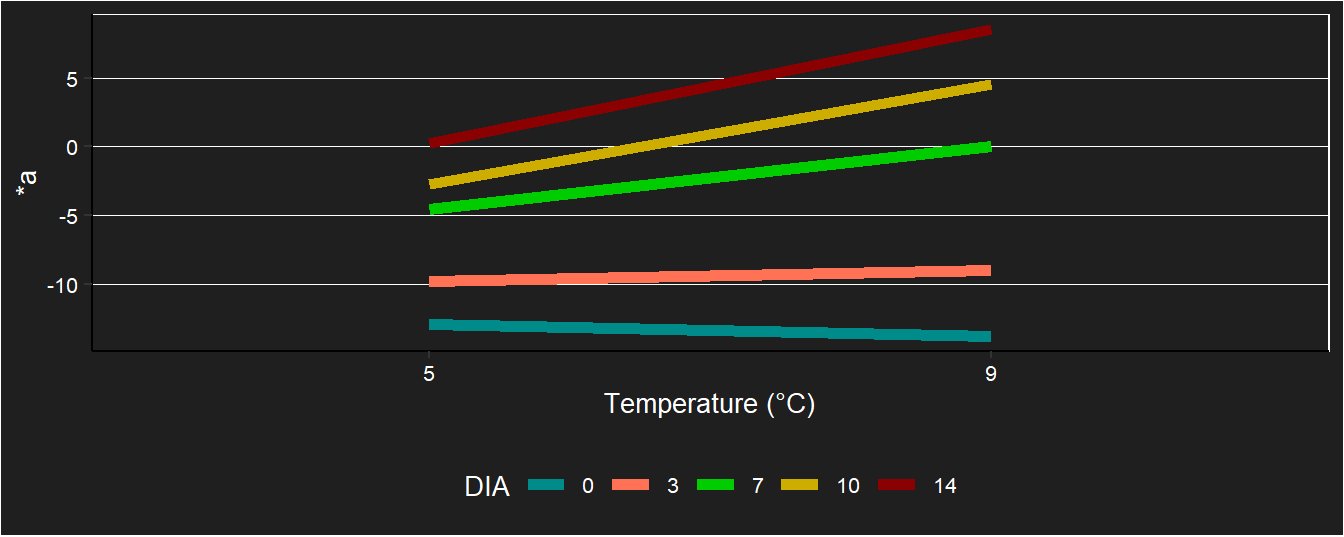
\includegraphics[width=0.95\linewidth]{madAcids_files/figure-latex/unnamed-chunk-36-2} \end{center}

\begin{verbatim}
## 
##  Shapiro-Wilk normality test
## 
## data:  e
## W = 0.7503611, p-value = 5.0413e-05
\end{verbatim}

Anova

\begin{verbatim}
##             numDF denDF    F-value p-value
## (Intercept)     1    18 10.6987231  0.0042
## MAD             3    18 26.0396084  <.0001
\end{verbatim}

Test de Tukey

\begin{verbatim}
## $emmeans
##  MAD      emmean          SE df     lower.CL    upper.CL
##  I   0.000000000 0.107480774  2 -0.462452447 0.462452447
##  MM  0.000000000 0.107480774  2 -0.462452447 0.462452447
##  M   0.000000000 0.107480774  2 -0.462452447 0.462452447
##  SM  0.941135667 0.107480774  2  0.478683220 1.403588114
## 
## Degrees-of-freedom method: containment 
## Confidence level used: 0.95 
## 
## $contrasts
##  contrast     estimate          SE df t.ratio p.value
##  I - MM    0.000000000 0.130412737 18   0.000  1.0000
##  I - M     0.000000000 0.130412737 18   0.000  1.0000
##  I - SM   -0.941135667 0.130412737 18  -7.217  <.0001
##  MM - M    0.000000000 0.130412737 18   0.000  1.0000
##  MM - SM  -0.941135667 0.130412737 18  -7.217  <.0001
##  M - SM   -0.941135667 0.130412737 18  -7.217  <.0001
## 
## Degrees-of-freedom method: containment 
## P value adjustment: tukey method for comparing a family of 4 estimates
\end{verbatim}

\begin{center}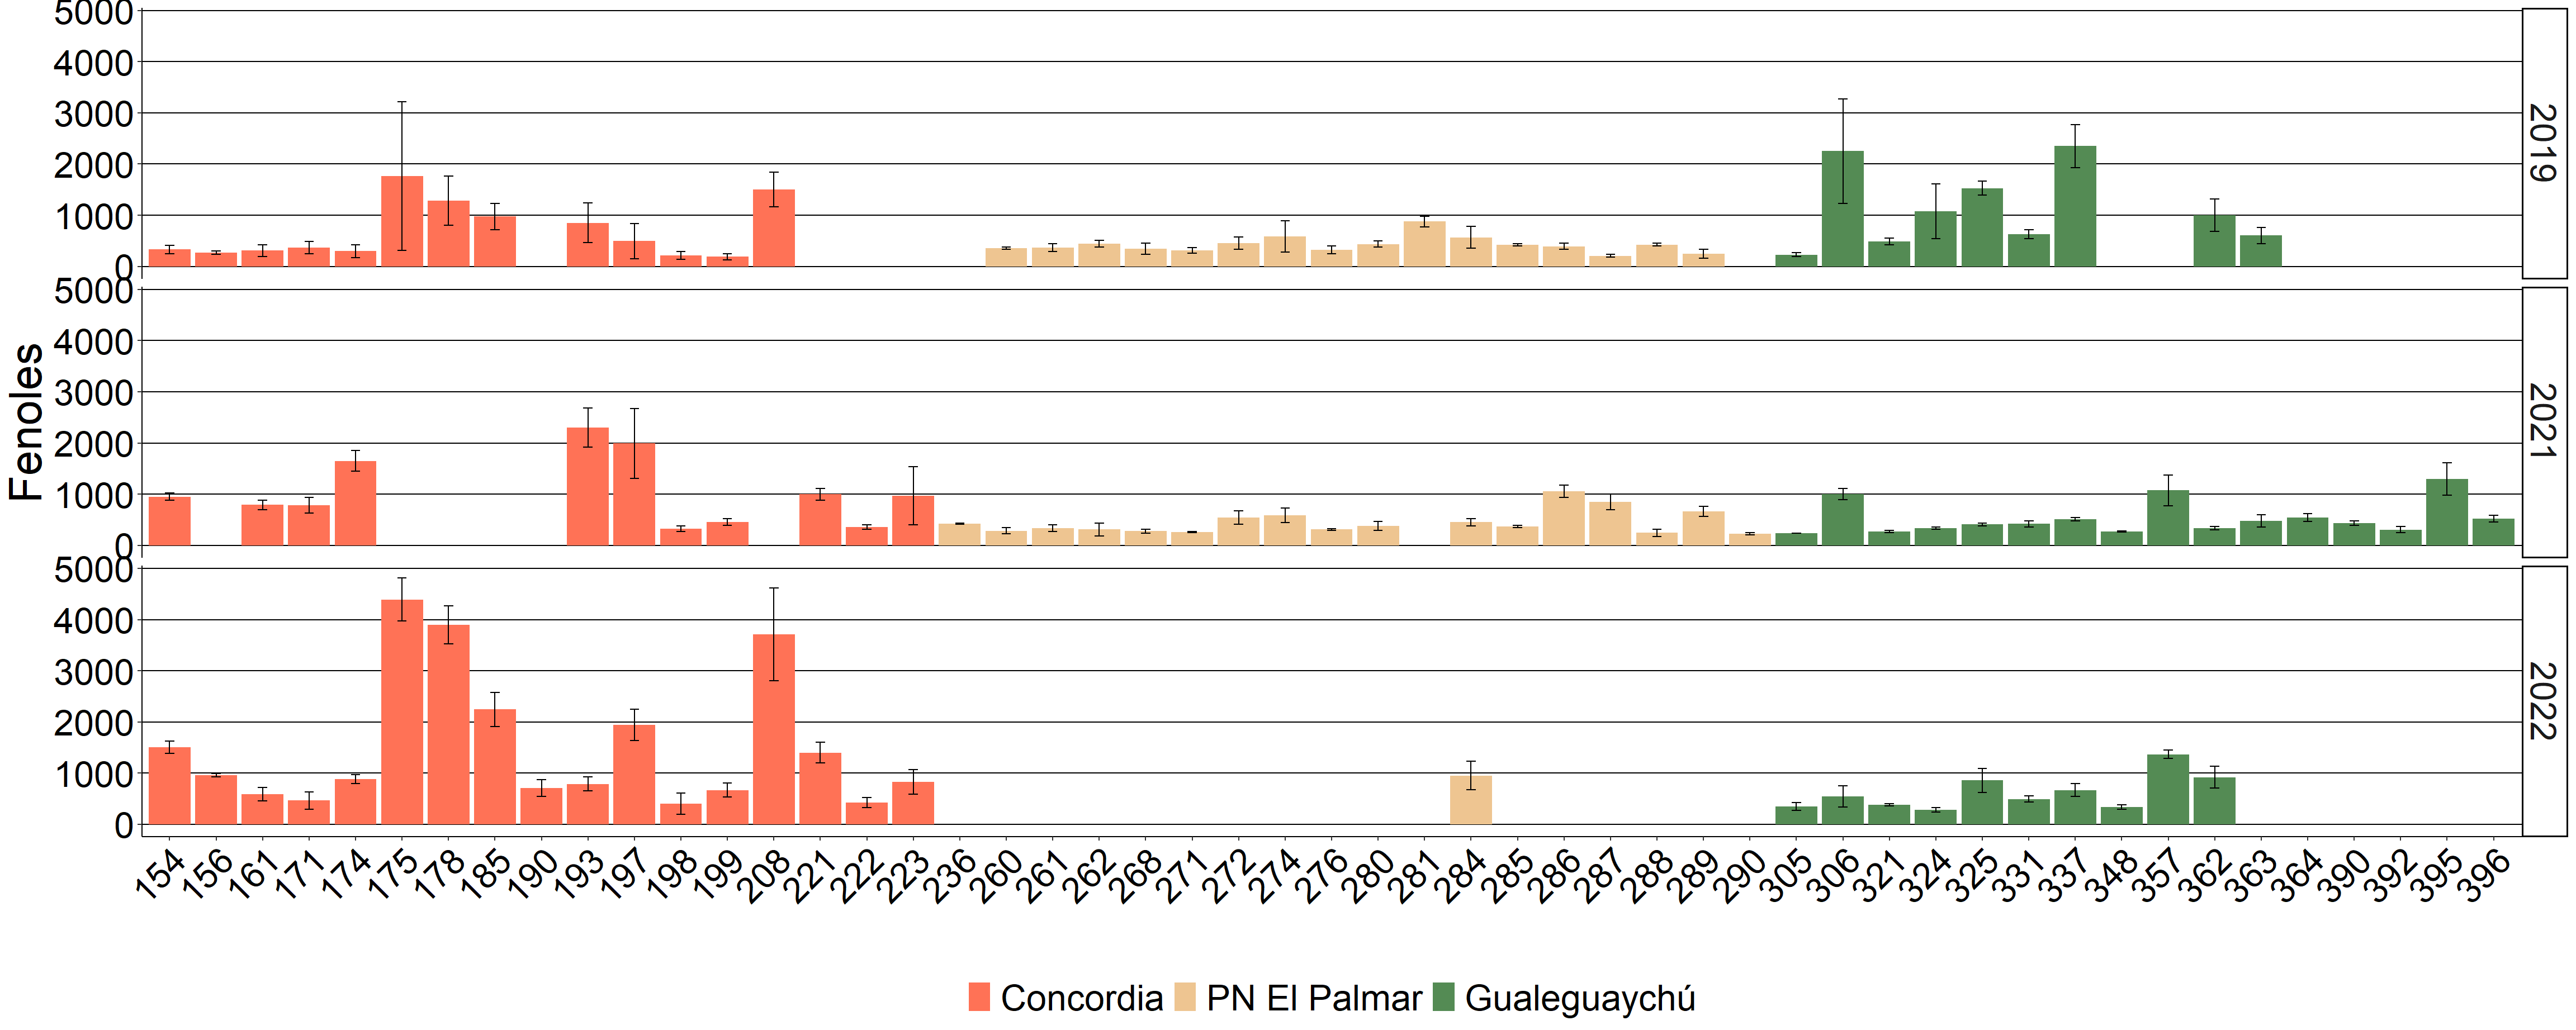
\includegraphics[width=0.95\linewidth]{madAcids_files/figure-latex/unnamed-chunk-38-1} \end{center}

\subsection{Ácido málico}\label{uxe1cido-muxe1lico-1}

Modelo y supuestos

\begin{verbatim}
## Linear mixed-effects model fit by REML
##   Data: mal 
##   Log-restricted-likelihood: -66.5285047
##   Fixed: CONS ~ MAD 
## (Intercept)       MADMM        MADM       MADSM 
##  44.9021340  45.2873977  60.2453557  39.8924652 
## 
## Random effects:
##  Formula: ~1 | REP
##         (Intercept)   Residual
## StdDev:  3.18440631 19.9143832
## 
## Variance function:
##  Structure: Different standard deviations per stratum
##  Formula: ~1 | MAD 
##  Parameter estimates:
##            I            M           MM           SM 
## 1.0000000000 0.0829966037 0.2681538614 0.1785082895 
## Number of Observations: 24
## Number of Groups: 3
\end{verbatim}

\begin{center}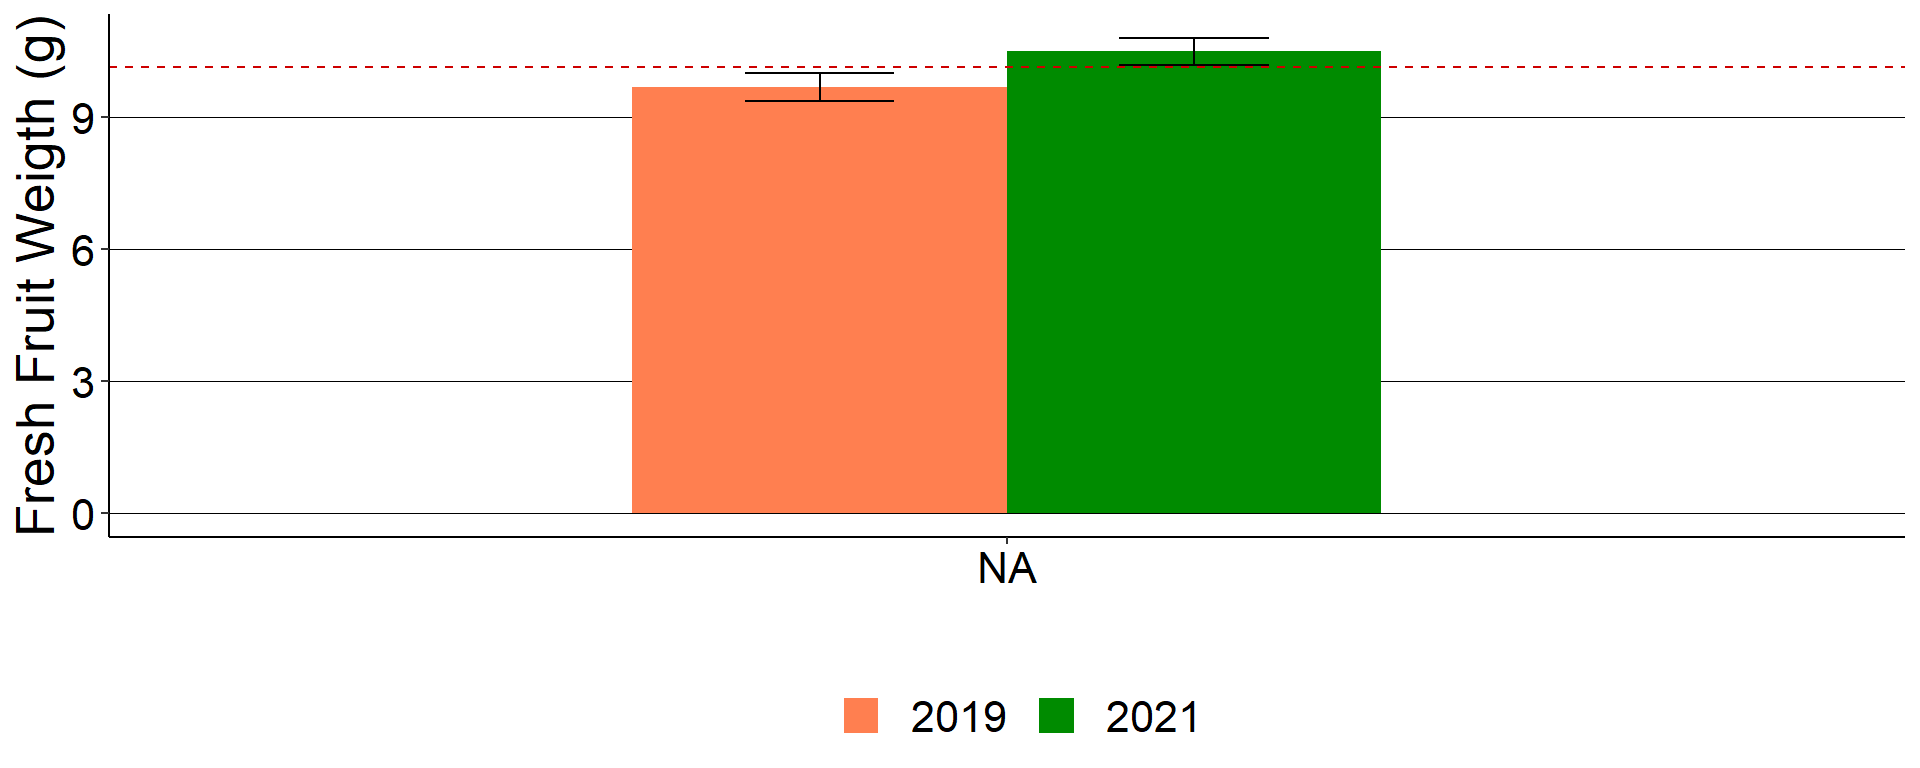
\includegraphics[width=0.95\linewidth]{madAcids_files/figure-latex/unnamed-chunk-40-1} \end{center}

\begin{center}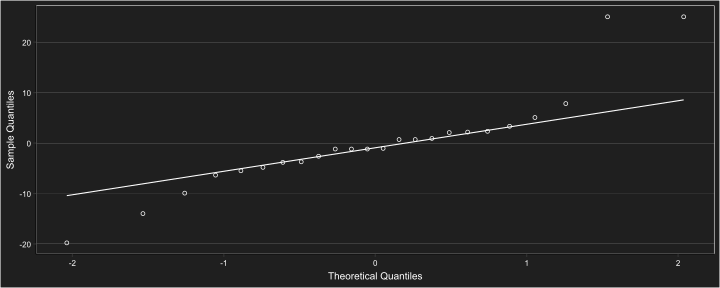
\includegraphics[width=0.95\linewidth]{madAcids_files/figure-latex/unnamed-chunk-40-2} \end{center}

\begin{verbatim}
## 
##  Shapiro-Wilk normality test
## 
## data:  e
## W = 0.872026, p-value = 0.00576551
\end{verbatim}

Anova

\begin{verbatim}
##             numDF denDF    F-value p-value
## (Intercept)     1    18 2706.36602  <.0001
## MAD             3    18   77.88670  <.0001
\end{verbatim}

Test de Tukey

\begin{verbatim}
## $emmeans
##  MAD      emmean         SE df   lower.CL    upper.CL
##  I    44.9021340 8.33530189  2  9.0382246  80.7660434
##  MM   90.1895317 2.85183436  2 77.9190788 102.4599846
##  M   105.1474897 1.95843141  2 96.7210394 113.5739399
##  SM   84.7945992 2.34229505  2 74.7165170  94.8726813
## 
## Degrees-of-freedom method: containment 
## Confidence level used: 0.95 
## 
## $contrasts
##  contrast    estimate         SE df t.ratio p.value
##  I - MM   -45.2873977 8.41723952 18  -5.380  0.0002
##  I - M    -60.2453557 8.15796638 18  -7.385  <.0001
##  I - SM   -39.8924652 8.25852940 18  -4.830  0.0007
##  MM - M   -14.9579580 2.28212995 18  -6.554  <.0001
##  MM - SM    5.3949325 2.61897110 18   2.060  0.2038
##  M - SM    20.3528905 1.60046992 18  12.717  <.0001
## 
## Degrees-of-freedom method: containment 
## P value adjustment: tukey method for comparing a family of 4 estimates
\end{verbatim}

\begin{center}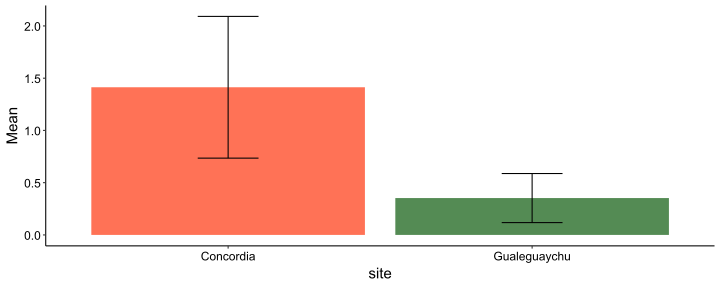
\includegraphics[width=0.95\linewidth]{madAcids_files/figure-latex/unnamed-chunk-42-1} \end{center}

\subsection{Ácido quínico}\label{uxe1cido-quuxednico-1}

Modelo y supuestos

\begin{verbatim}
## Linear mixed-effects model fit by REML
##   Data: qui 
##   Log-restricted-likelihood: 58.1548863
##   Fixed: CONS ~ MAD 
##  (Intercept)        MADMM         MADM        MADSM 
##  0.374677755 24.876943000 22.248144833 22.479761167 
## 
## Random effects:
##  Formula: ~1 | REP
##         (Intercept)       Residual
## StdDev: 0.671027165 1.17940857e-16
## 
## Variance function:
##  Structure: Different standard deviations per stratum
##  Formula: ~1 | MAD 
##  Parameter estimates:
##              I              M             MM             SM 
## 1.00000000e+00 2.22331623e+16 3.72325836e+16 3.66668232e+16 
## Number of Observations: 24
## Number of Groups: 3
\end{verbatim}

\begin{center}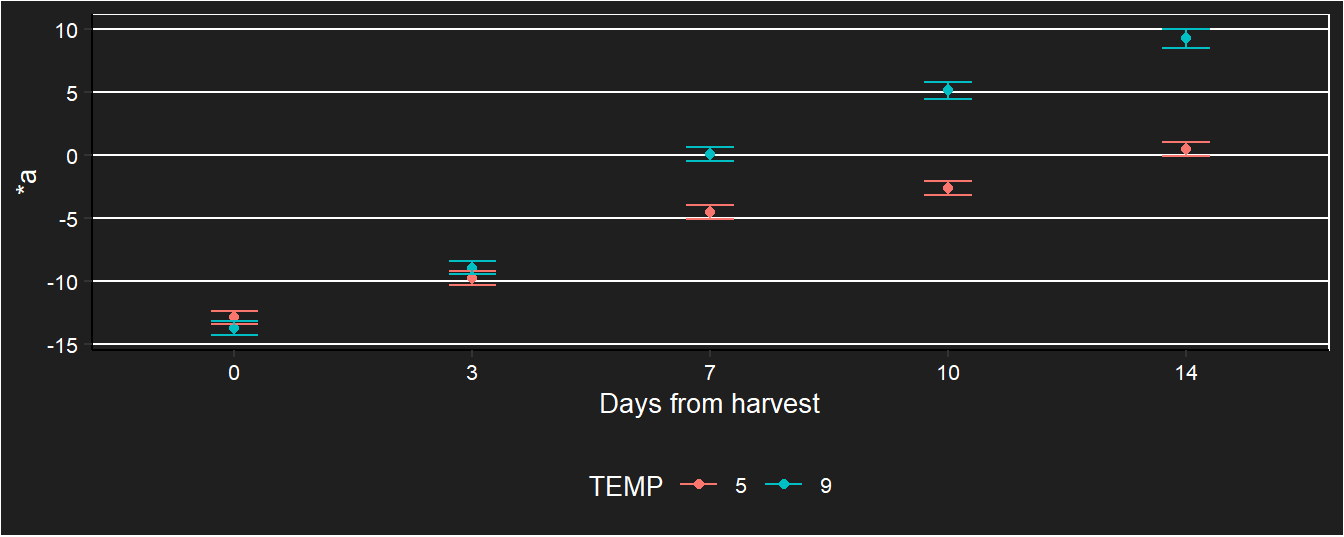
\includegraphics[width=0.95\linewidth]{madAcids_files/figure-latex/unnamed-chunk-45-1} \end{center}

\begin{center}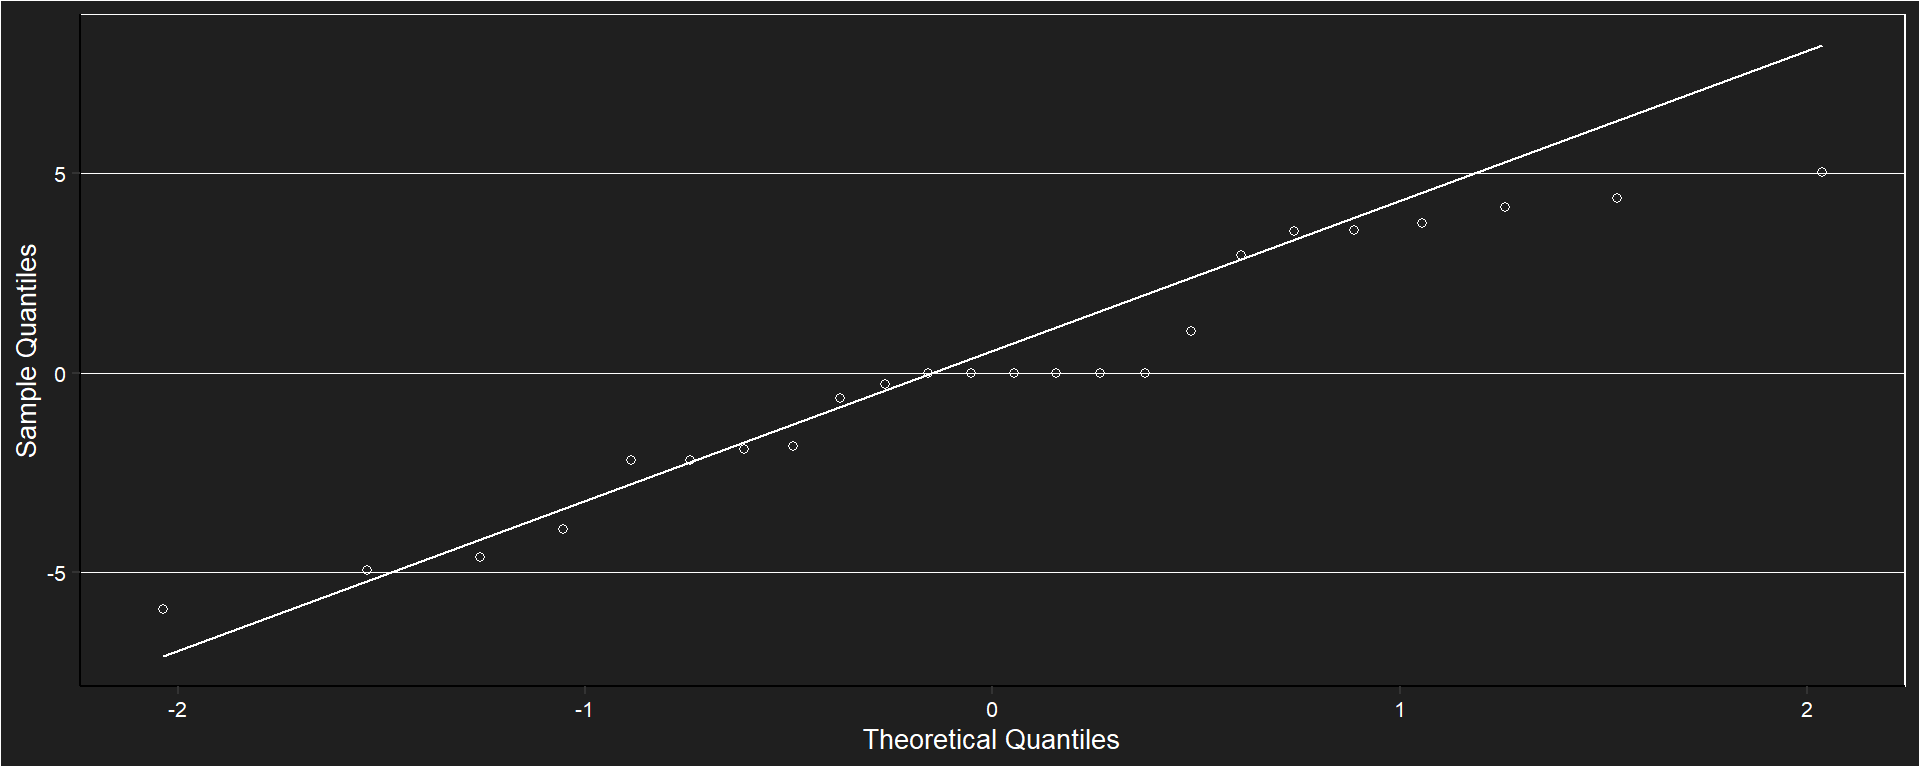
\includegraphics[width=0.95\linewidth]{madAcids_files/figure-latex/unnamed-chunk-45-2} \end{center}

\begin{verbatim}
## 
##  Shapiro-Wilk normality test
## 
## data:  e
## W = 0.9457795, p-value = 0.219116
\end{verbatim}

Anova

\begin{verbatim}
##             numDF denDF     F-value p-value
## (Intercept)     1    18   2.4280693  0.1366
## MAD             3    18 262.2049802  <.0001
\end{verbatim}

Test de Tukey

\begin{verbatim}
## $emmeans
##  MAD      emmean          SE df    lower.CL   upper.CL
##  I    0.37467776 0.240451435  2 -0.65990127  1.4092568
##  MM  25.25162076 1.808770981  2 17.46910736 33.0341342
##  M   22.62282259 1.097180084  2 17.90203771 27.3436075
##  SM  22.85443892 1.781775553  2 15.18807748 30.5208004
## 
## Degrees-of-freedom method: containment 
## Confidence level used: 0.95 
## 
## $contrasts
##  contrast     estimate         SE df t.ratio p.value
##  I - MM   -24.87694300 1.79271737 18 -13.877  <.0001
##  I - M    -22.24814483 1.07050794 18 -20.783  <.0001
##  I - SM   -22.47976117 1.76547649 18 -12.733  <.0001
##  MM - M     2.62879817 2.08801887 18   1.259  0.5992
##  MM - SM    2.39718183 2.51609674 18   0.953  0.7772
##  M - SM    -0.23161633 2.06467781 18  -0.112  0.9995
## 
## Degrees-of-freedom method: containment 
## P value adjustment: tukey method for comparing a family of 4 estimates
\end{verbatim}

\begin{center}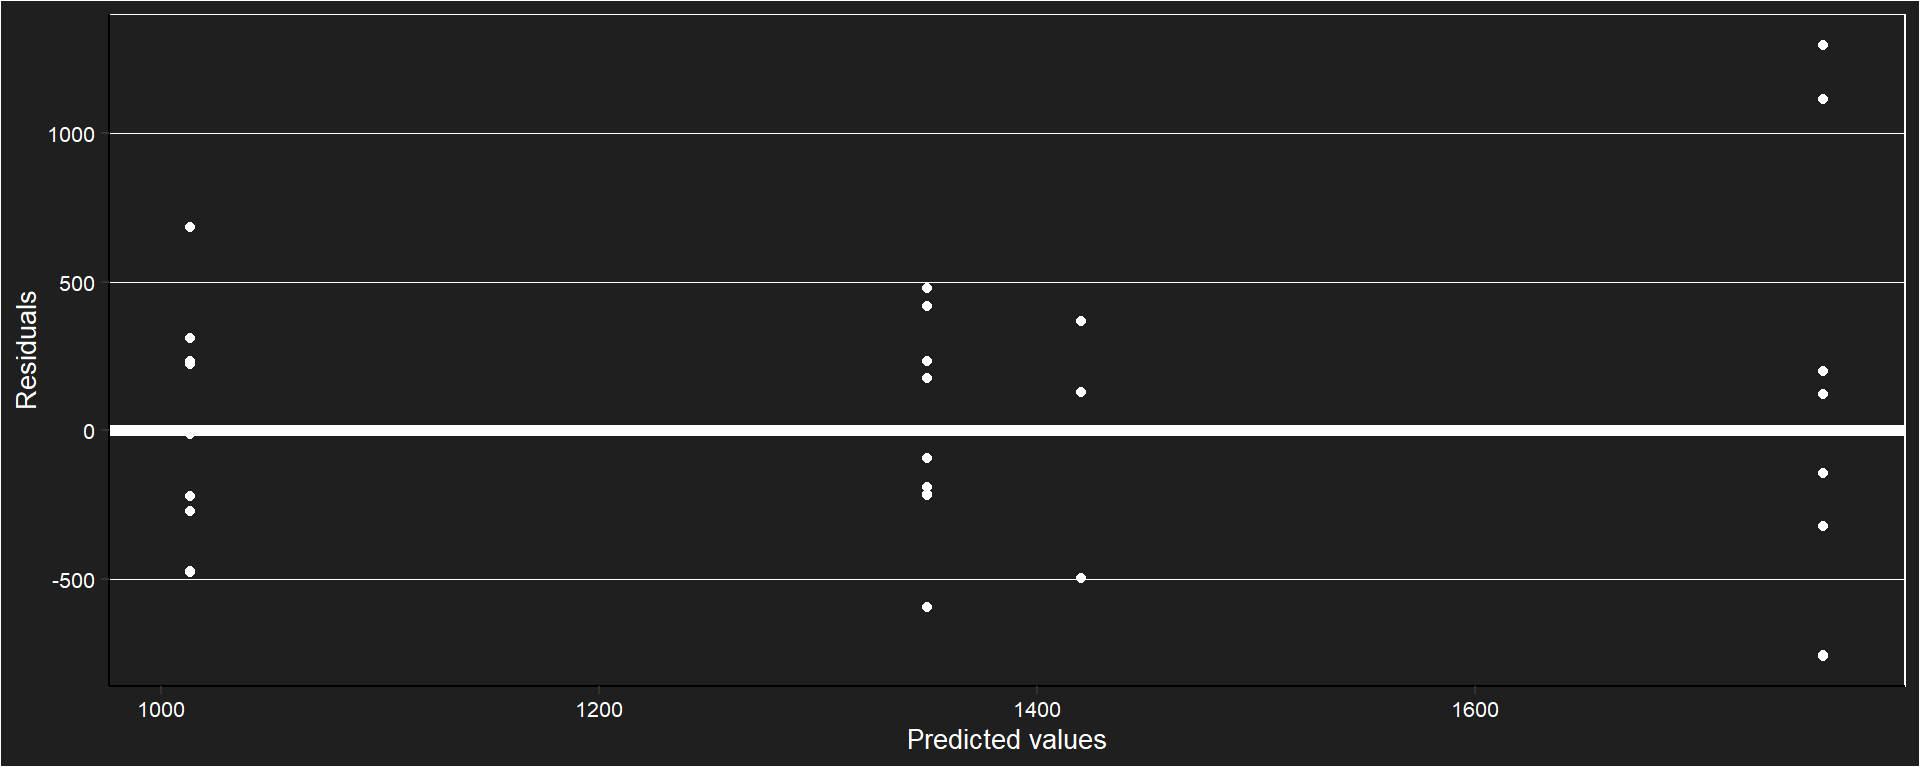
\includegraphics[width=0.95\linewidth]{madAcids_files/figure-latex/unnamed-chunk-47-1} \end{center}

\subsection{Ácido succinico}\label{uxe1cido-succinico-1}

Modelo y supuestos

\begin{verbatim}
## Linear mixed-effects model fit by REML
##   Data: suc 
##   Log-restricted-likelihood: -72.9162935
##   Fixed: CONS ~ MAD 
##  (Intercept)        MADMM         MADM        MADSM 
## 112.33348650 -19.85189417 -12.89624667   3.32166483 
## 
## Random effects:
##  Formula: ~1 | REP
##         (Intercept)   Residual
## StdDev:  2.08906489 7.56778496
## 
## Number of Observations: 24
## Number of Groups: 3
\end{verbatim}

\begin{center}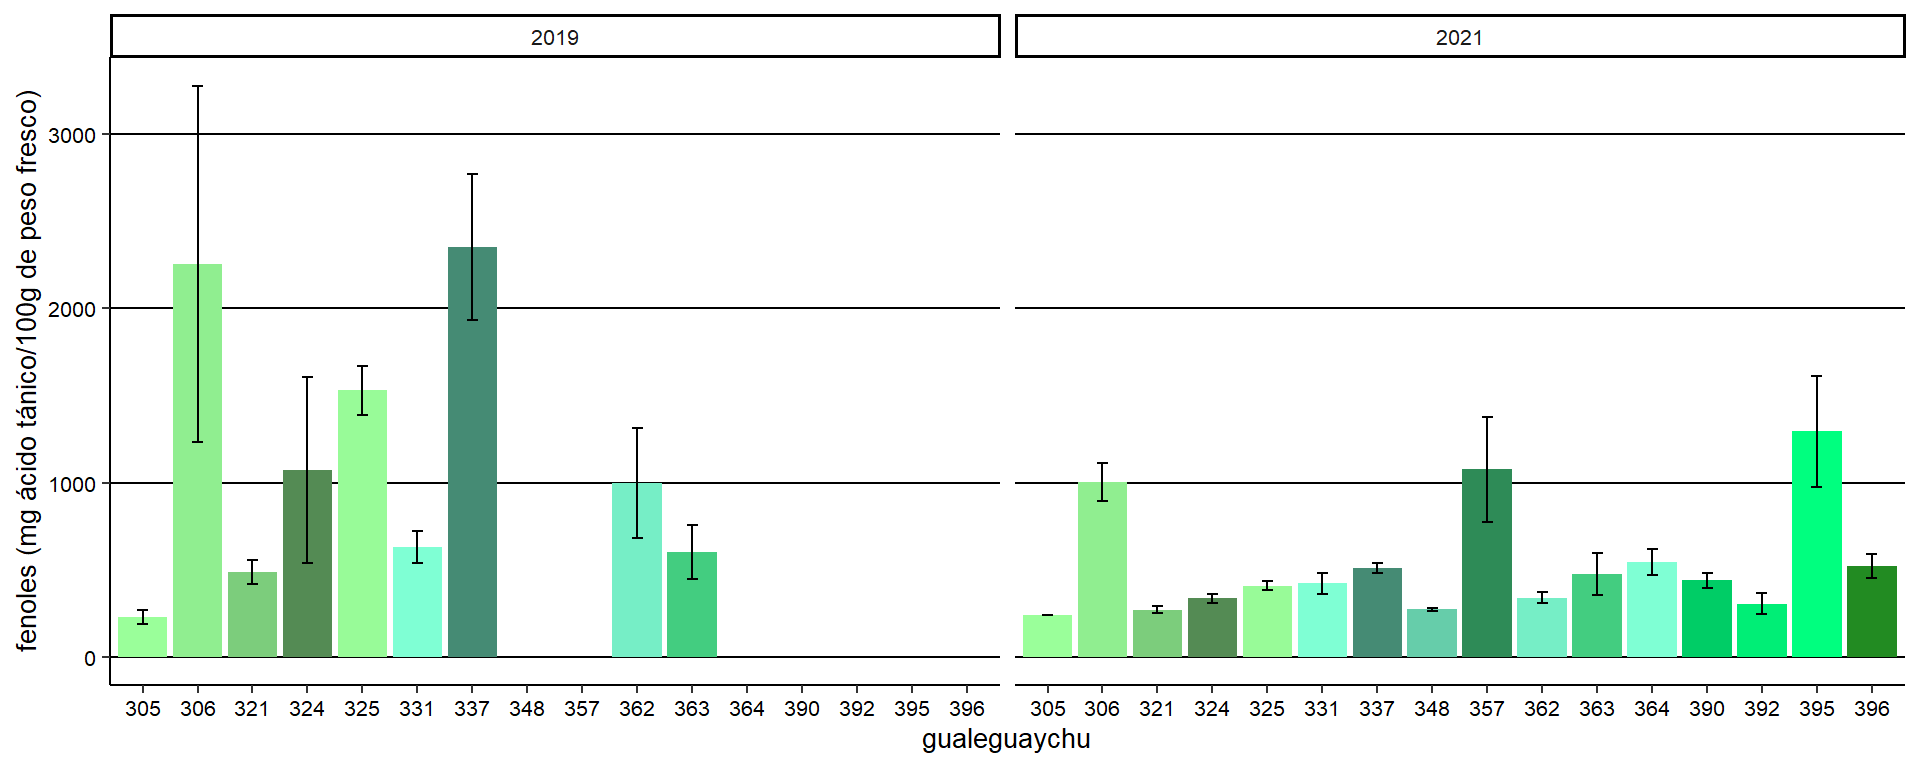
\includegraphics[width=0.95\linewidth]{madAcids_files/figure-latex/unnamed-chunk-48-1} \end{center}

\begin{center}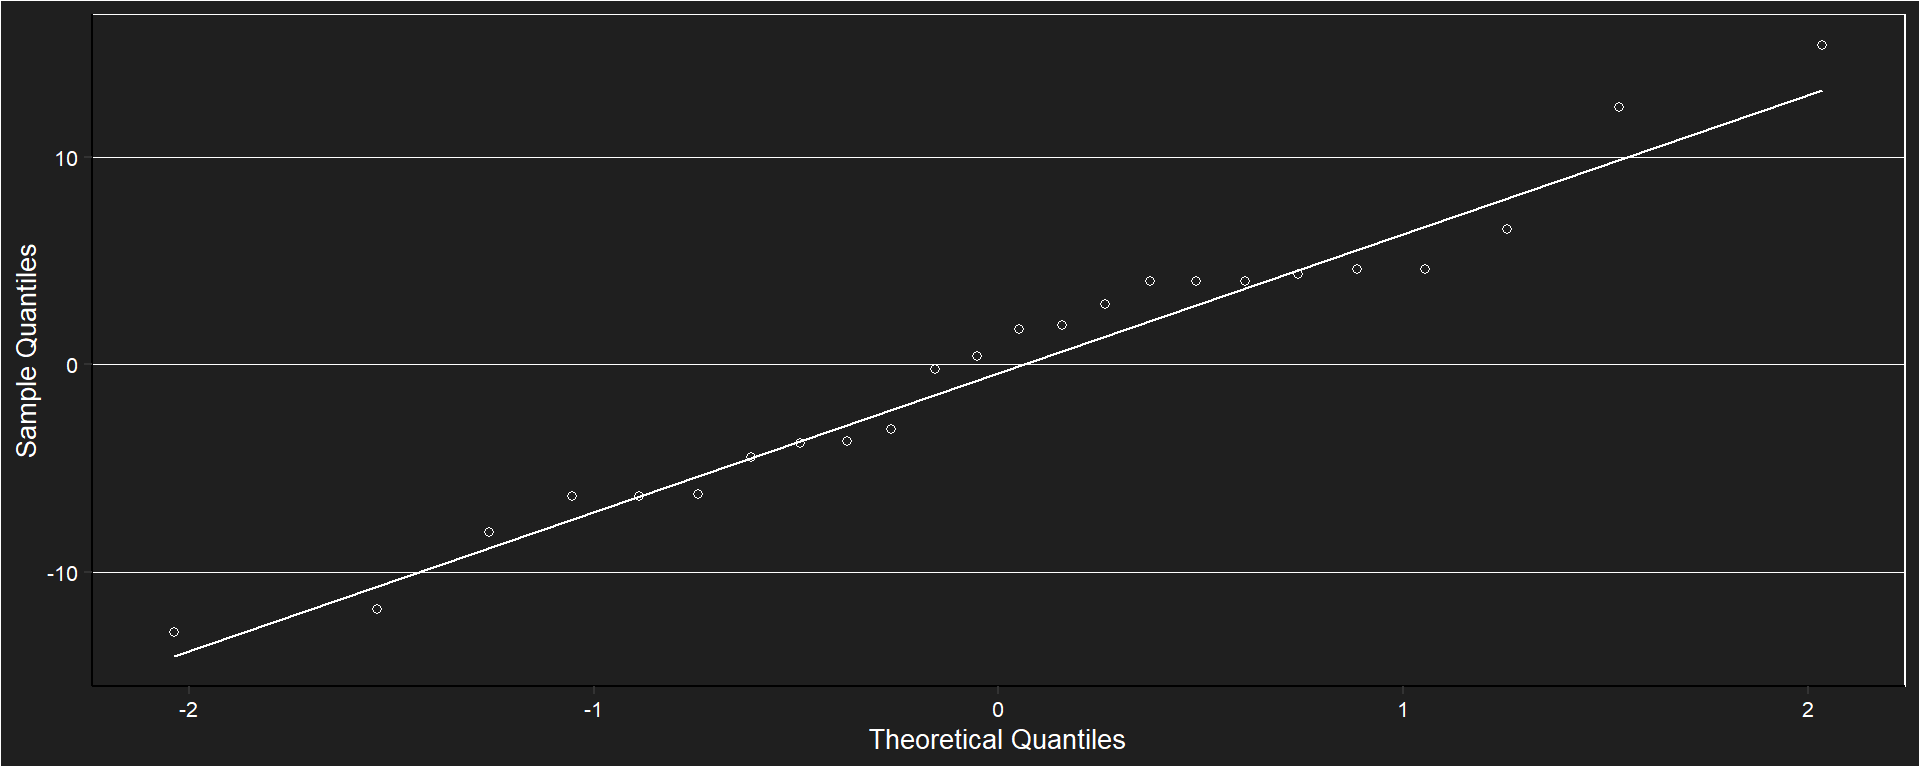
\includegraphics[width=0.95\linewidth]{madAcids_files/figure-latex/unnamed-chunk-48-2} \end{center}

\begin{verbatim}
## 
##  Shapiro-Wilk normality test
## 
## data:  e
## W = 0.9675281, p-value = 0.606483
\end{verbatim}

\begin{verbatim}
## Levene's Test for Homogeneity of Variance (center = median)
##       Df F value  Pr(>F)
## group  3 1.48182 0.24974
##       20
\end{verbatim}

Anova

\begin{verbatim}
##             numDF denDF     F-value p-value
## (Intercept)     1    18 2869.053469  <.0001
## MAD             3    18   12.395896   1e-04
\end{verbatim}

Test de Tukey

\begin{verbatim}
## $emmeans
##  MAD      emmean        SE df    lower.CL   upper.CL
##  I   112.3334865 3.3166186  2  98.0632284 126.603745
##  MM   92.4815923 3.3166186  2  78.2113343 106.751850
##  M    99.4372398 3.3166186  2  85.1669818 113.707498
##  SM  115.6551513 3.3166186  2 101.3848933 129.925409
## 
## Degrees-of-freedom method: containment 
## Confidence level used: 0.95 
## 
## $contrasts
##  contrast     estimate         SE df t.ratio p.value
##  I - MM    19.85189417 4.36926268 18   4.544  0.0013
##  I - M     12.89624667 4.36926268 18   2.952  0.0389
##  I - SM    -3.32166483 4.36926268 18  -0.760  0.8711
##  MM - M    -6.95564750 4.36926268 18  -1.592  0.4076
##  MM - SM  -23.17355900 4.36926268 18  -5.304  0.0003
##  M - SM   -16.21791150 4.36926268 18  -3.712  0.0079
## 
## Degrees-of-freedom method: containment 
## P value adjustment: tukey method for comparing a family of 4 estimates
\end{verbatim}

\begin{center}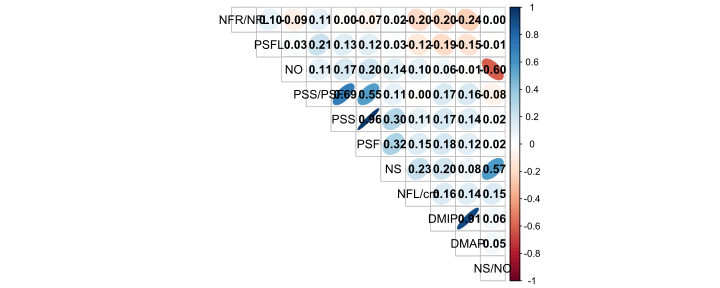
\includegraphics[width=0.95\linewidth]{madAcids_files/figure-latex/unnamed-chunk-50-1} \end{center}

\subsection{Relación de ácidos orgánicos y acidez total titulable
ATT.}\label{relaciuxf3n-de-uxe1cidos-orguxe1nicos-y-acidez-total-titulable-att.}

\begin{verbatim}
##          CAR MAD N          CONS            sd            se            ci
## 1  Tartárico   I 6   0.000000000  0.0000000000  0.0000000000  0.0000000000
## 2  Tartárico  MM 6   0.000000000  0.0000000000  0.0000000000  0.0000000000
## 3  Tartárico   M 6   0.000000000  0.0000000000  0.0000000000  0.0000000000
## 4  Tartárico  SM 6   0.941135667  0.4830674796  0.1972114727  0.5069482296
## 5     Málico   I 6  44.902134000 19.1523848051  7.8189283550 20.0991952034
## 6     Málico  MM 6  90.189531667  4.0220151138  1.6419807944  4.2208460046
## 7     Málico   M 6 105.147489667  3.3635751544  1.3731738066  3.5298556445
## 8     Málico  SM 6  84.794599167  5.3680332445  2.1914903952  5.6334054030
## 9    Quínico   I 6   0.440663333  0.6826727005  0.2786999629  0.7164210623
## 10   Quínico  MM 6  25.317606333  3.8140013880  1.5570595465  4.0025489871
## 11   Quínico   M 6  22.688808167  2.2426216210  0.9155464429  2.3534870559
## 12   Quínico  SM 6  22.920424500  3.7568053163  1.5337093480  3.9425253911
## 13 Succínico   I 6 112.333486500  6.5345265736  2.6677093027  6.8575650762
## 14 Succínico  MM 6  92.481592333  4.7805090422  1.9516346440  5.0168365657
## 15 Succínico   M 6  99.437239833  4.8240138759  1.9693954180  5.0624920887
## 16 Succínico  SM 6 115.655151333 12.4187930831  5.0699510458 13.0327240659
## 17       ATT   I 3   1.779200000  0.0507984252  0.0293284844  0.1261902837
## 18       ATT  MM 3   1.606400000  0.0278969532  0.0161063135  0.0692998736
## 19       ATT   M 3   1.828266667  0.2039063837  0.1177254055  0.5065315375
## 20       ATT  SM 3   1.384533333  0.0835275603  0.0482246594  0.2074939626
## 21   TOTALac   I 6 157.676283833 24.4147956495  9.9672985859 25.6217566954
## 22   TOTALac  MM 6 207.988730333 11.6569574255  4.7589329410 12.2332265750
## 23   TOTALac   M 6 227.273537667  4.2846255274  1.7491910468  4.4964387320
## 24   TOTALac  SM 6 224.311310667 13.9874059778  5.7103345784 14.6788823428
## 25      <NA>   I 6 266.880791667  8.4819431471  3.4627387896  8.9012534341
## 26      <NA>  MM 6 301.680354667 34.6167224669 14.1322177686 36.3280222931
## 27      <NA>   M 6 350.625756167 31.1823867560 12.7301560857 32.7239079987
## 28      <NA>  SM 6 428.368083167 26.7527791069 10.9217763355 28.0753198610
## 29     ACIDS   I 6 157.676283833 24.4147956495  9.9672985859 25.6217566954
## 30     ACIDS  MM 6 207.988730167 11.6569573346  4.7589329039 12.2332264797
## 31     ACIDS   M 6 227.273537833  4.2846256099  1.7491910805  4.4964388186
## 32     ACIDS  SM 6 224.311310667 13.9874058096  5.7103345098 14.6788821663
\end{verbatim}

Concentración del ratio azúcares totales / ácidos orgánicos totales a
distintos estados.

\begin{center}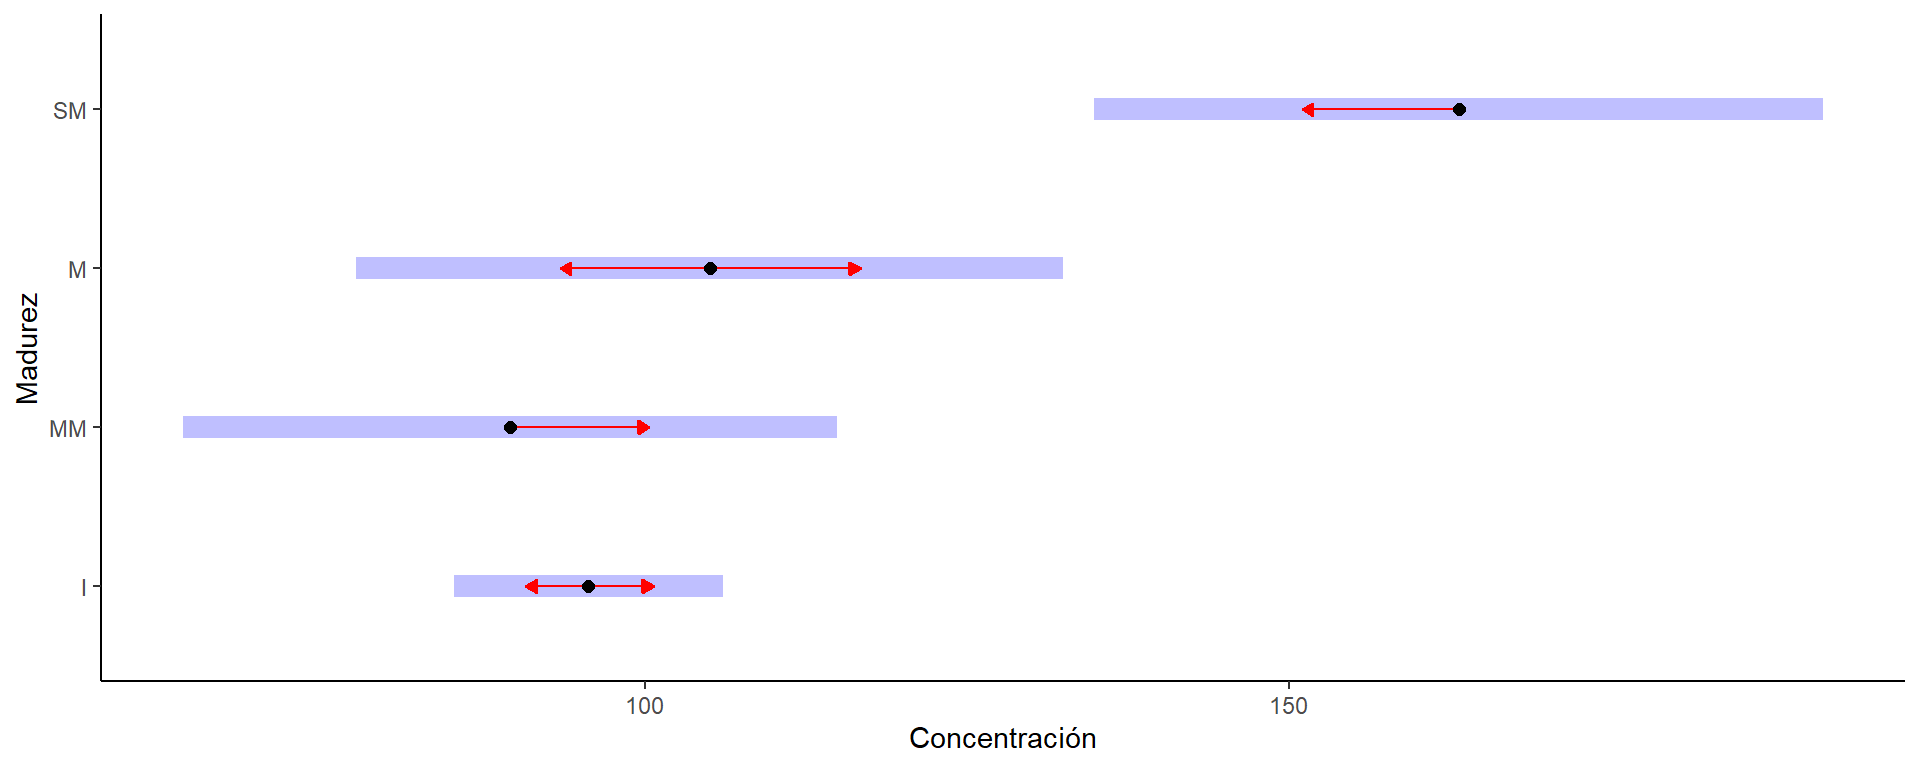
\includegraphics[width=0.95\linewidth]{madAcids_files/figure-latex/unnamed-chunk-52-1} \end{center}

Tabla descriptiva totales

\begin{verbatim}
##   MAD N     TOTALS            sd            se           ci
## 1   I 3 1.72112247 0.26333177284 0.15203466994 0.6541523876
## 2  MM 3 1.44765169 0.11629091852 0.06714059311 0.2888826562
## 3   M 3 1.54171591 0.13269129972 0.07660935761 0.3296234617
## 4  SM 3 1.90950427 0.00773336868 0.00446486249 0.0192107528
\end{verbatim}

Relación ST/AT (azúcares totales / ácidos totales)

\begin{verbatim}
## Linear mixed-effects model fit by REML
##   Data: dataSTAT 
##   Log-restricted-likelihood: 1.18539612
##   Fixed: TOTALS ~ MAD 
##  (Intercept)        MADMM         MADM        MADSM 
##  1.721122474 -0.273470784 -0.179406567  0.188381795 
## 
## Random effects:
##  Formula: ~1 | REP
##            (Intercept)    Residual
## StdDev: 0.000999703726 0.158534031
## 
## Number of Observations: 12
## Number of Groups: 3
\end{verbatim}

\begin{center}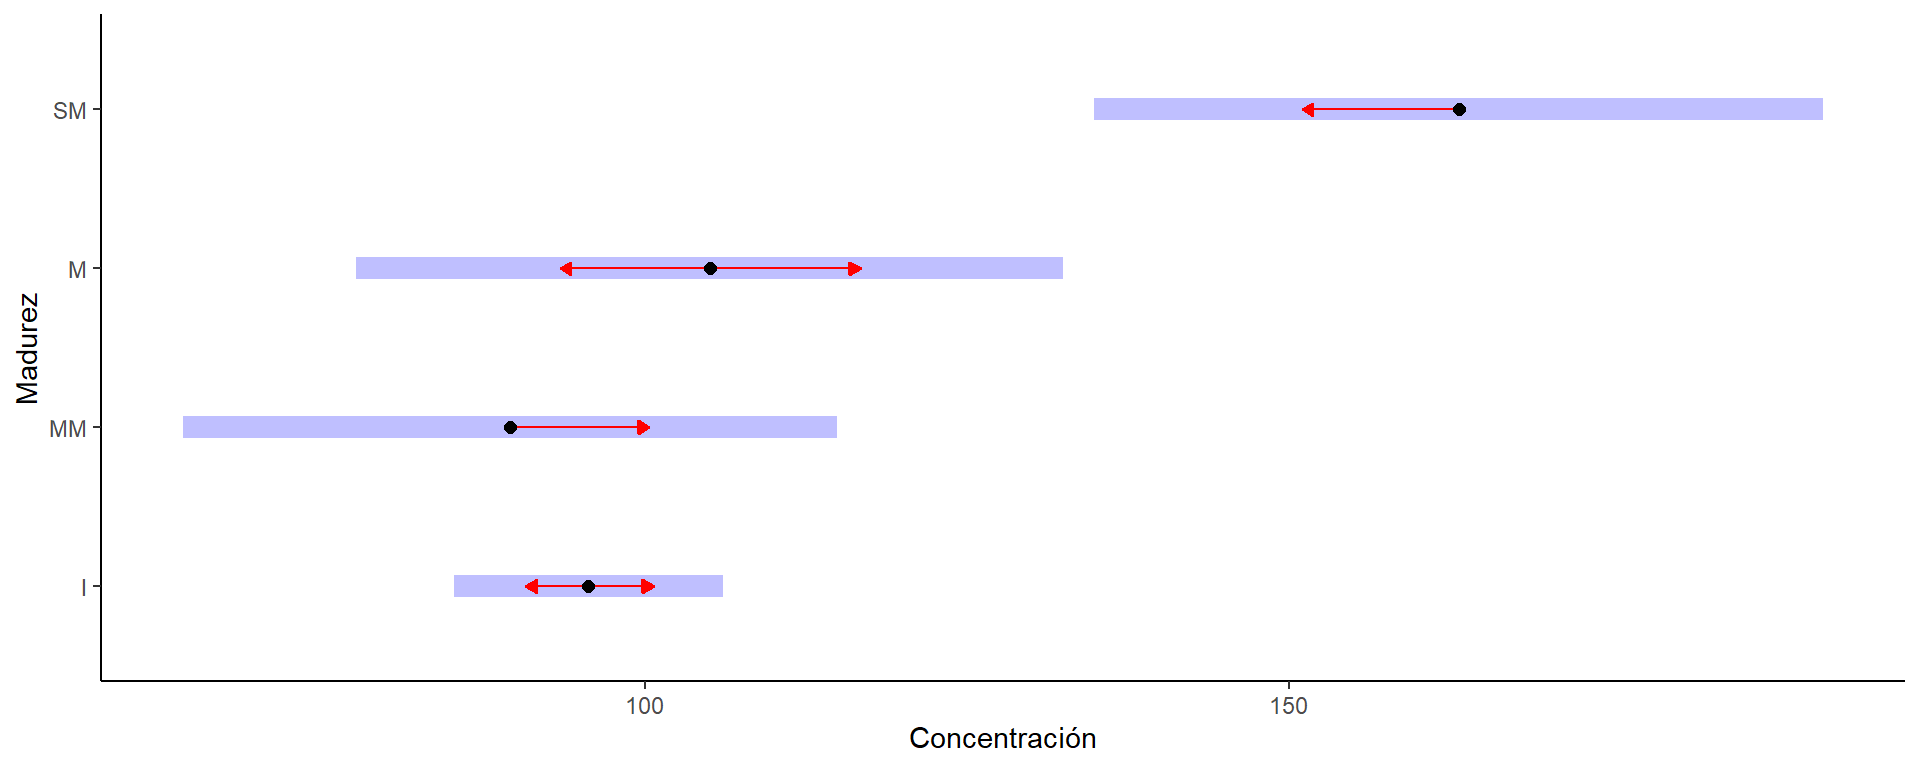
\includegraphics[width=0.95\linewidth]{madAcids_files/figure-latex/unnamed-chunk-54-1} \end{center}

\begin{center}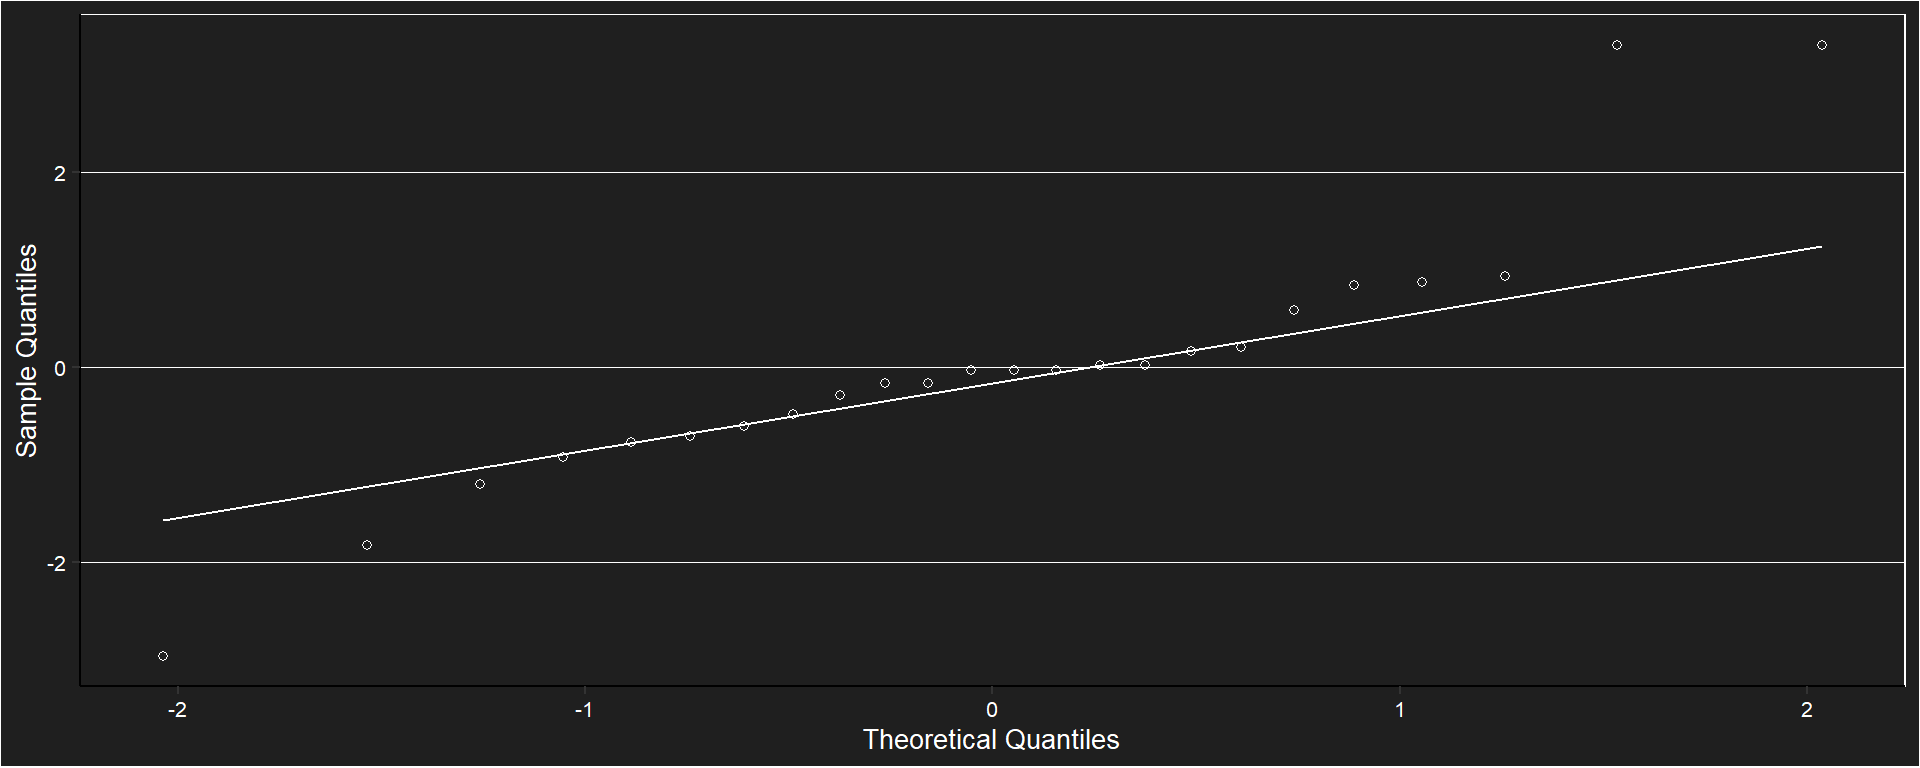
\includegraphics[width=0.95\linewidth]{madAcids_files/figure-latex/unnamed-chunk-54-2} \end{center}

\begin{verbatim}
## 
##  Shapiro-Wilk normality test
## 
## data:  e
## W = 0.9262267, p-value = 0.341827
\end{verbatim}

Anova

\begin{verbatim}
##             numDF denDF     F-value p-value
## (Intercept)     1     6 1307.562391  <.0001
## MAD             3     6    4.972388  0.0457
\end{verbatim}

Test de Tukey

\begin{verbatim}
## $emmeans
##  MAD     emmean           SE df   lower.CL   upper.CL
##  I   1.72112247 0.0915314854  2 1.32729428 2.11495067
##  MM  1.44765169 0.0915314854  2 1.05382350 1.84147989
##  M   1.54171591 0.0915314854  2 1.14788771 1.93554410
##  SM  1.90950427 0.0915314854  2 1.51567607 2.30333246
## 
## Degrees-of-freedom method: containment 
## Confidence level used: 0.95 
## 
## $contrasts
##  contrast     estimate          SE df t.ratio p.value
##  I - MM    0.273470784 0.129442495  6   2.113  0.2498
##  I - M     0.179406567 0.129442495  6   1.386  0.5497
##  I - SM   -0.188381795 0.129442495  6  -1.455  0.5142
##  MM - M   -0.094064217 0.129442495  6  -0.727  0.8831
##  MM - SM  -0.461852579 0.129442495  6  -3.568  0.0443
##  M - SM   -0.367788362 0.129442495  6  -2.841  0.1041
## 
## Degrees-of-freedom method: containment 
## P value adjustment: tukey method for comparing a family of 4 estimates
\end{verbatim}

\begin{center}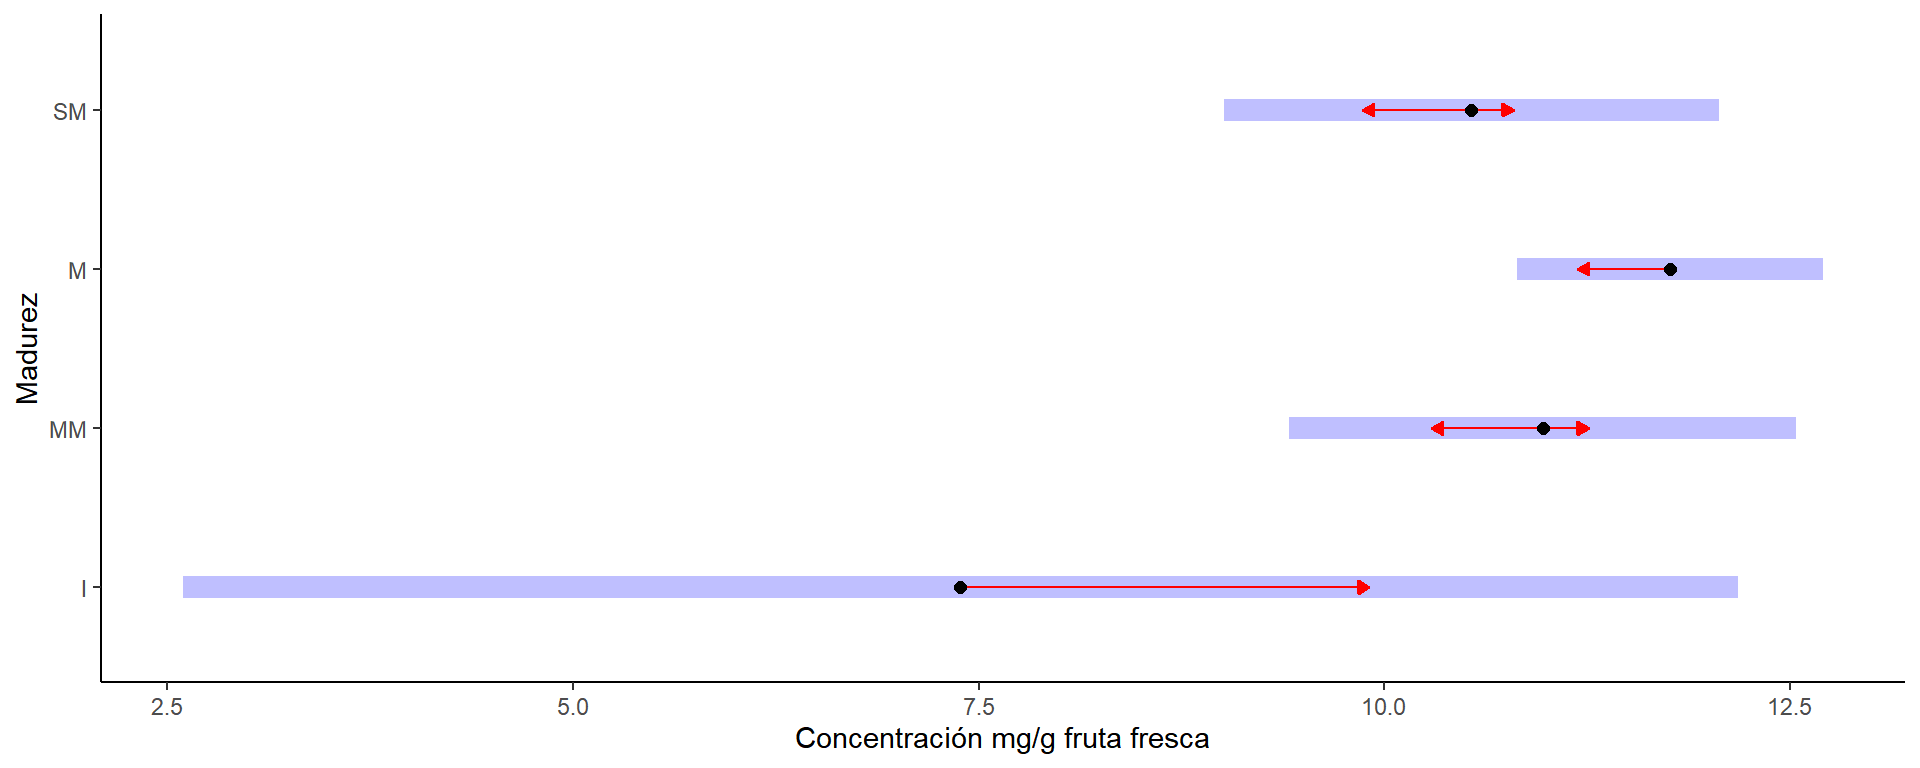
\includegraphics[width=0.95\linewidth]{madAcids_files/figure-latex/unnamed-chunk-56-1} \end{center}

\subsection{Correlaciones}\label{correlaciones}

Correlaciones de Pearson.

\begin{center}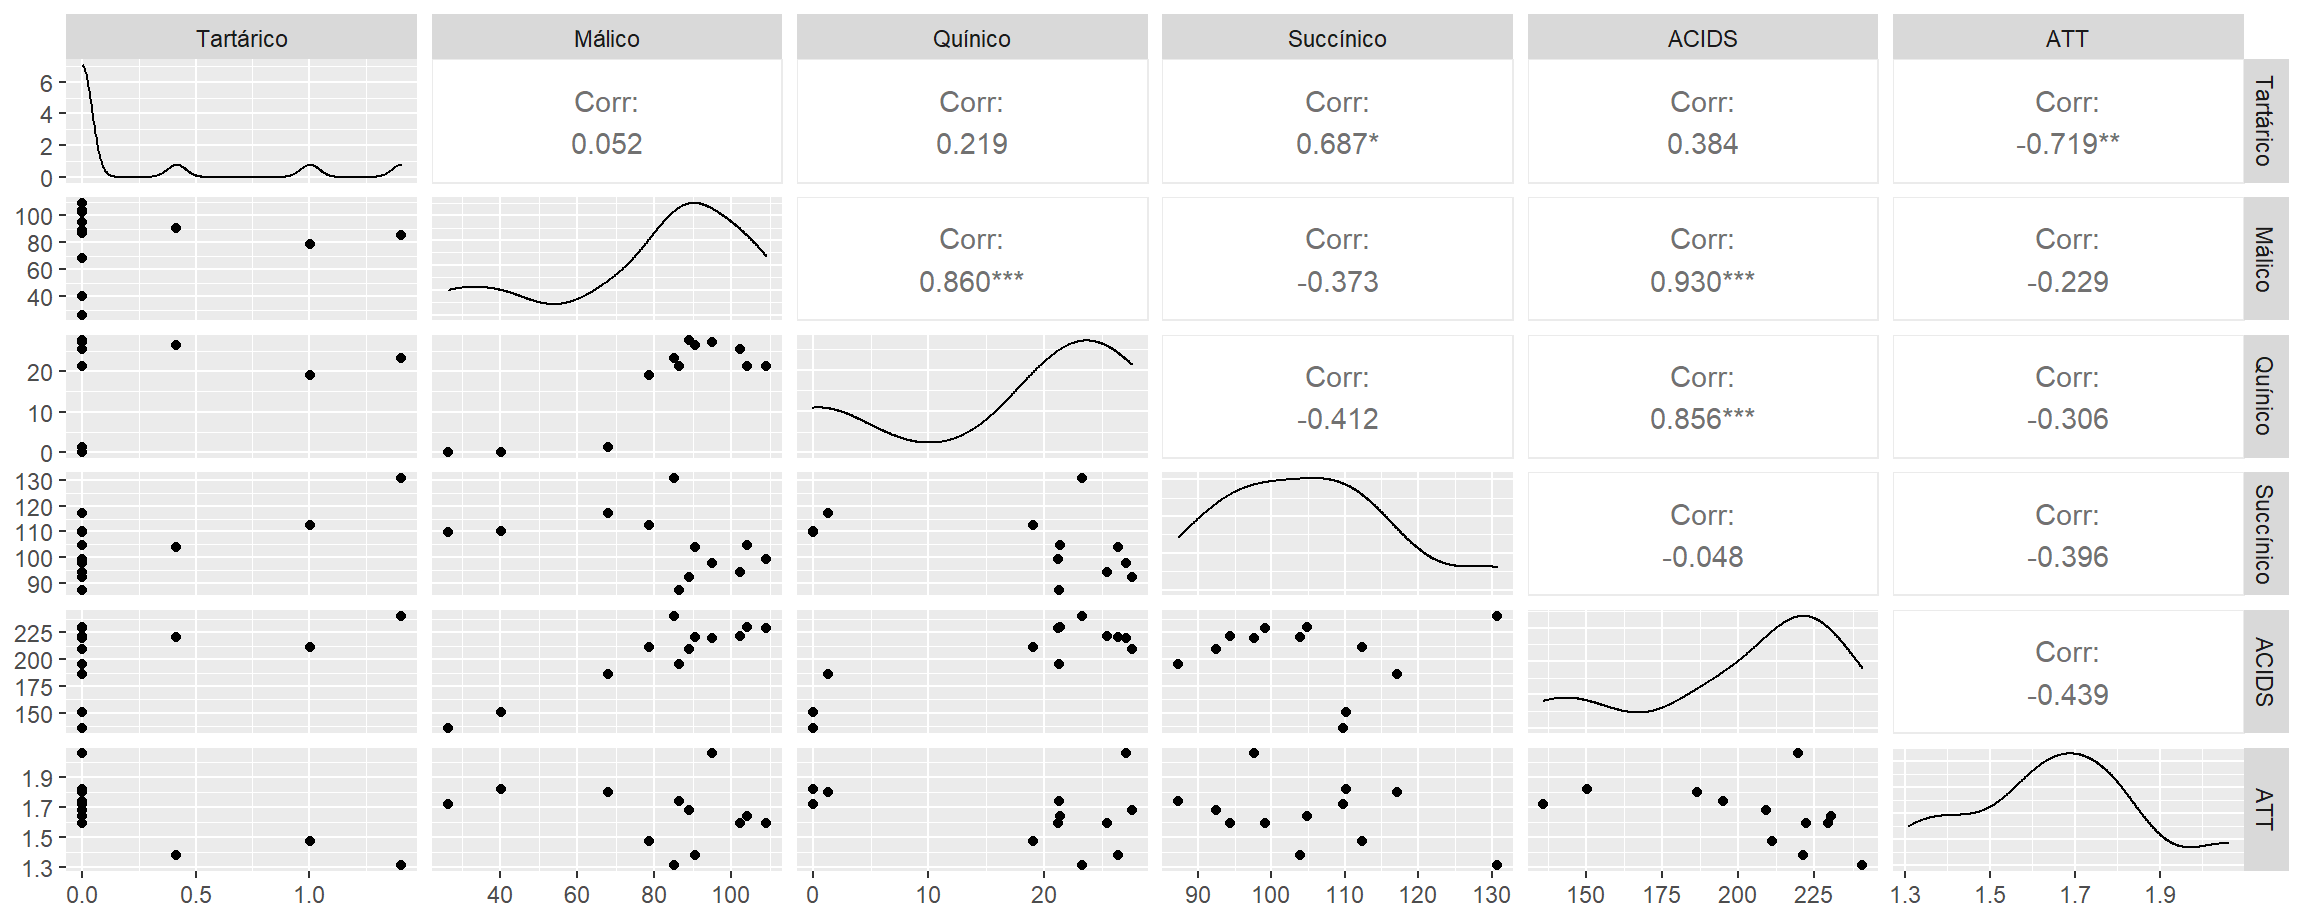
\includegraphics[width=0.95\linewidth]{madAcids_files/figure-latex/unnamed-chunk-58-1} \end{center}

\begin{verbatim}
## 
##  Pearson's product-moment correlation
## 
## data:  FACO$Málico and FACO$Quínico
## t = 5.329902, df = 10, p-value = 0.000333007
## alternative hypothesis: true correlation is not equal to 0
## 95 percent confidence interval:
##  0.564971048 0.960065608
## sample estimates:
##         cor 
## 0.860021264
\end{verbatim}

\begin{verbatim}
## 
##  Pearson's product-moment correlation
## 
## data:  FACO$Tartárico and FACO$Succínico
## t = 2.989547, df = 10, p-value = 0.0135842
## alternative hypothesis: true correlation is not equal to 0
## 95 percent confidence interval:
##  0.186681215 0.904338855
## sample estimates:
##         cor 
## 0.686981893
\end{verbatim}

\begin{verbatim}
## 
##  Pearson's product-moment correlation
## 
## data:  FACO$ATT and FACO$Tartárico
## t = -3.268633, df = 10, p-value = 0.00844982
## alternative hypothesis: true correlation is not equal to 0
## 95 percent confidence interval:
##  -0.915141012 -0.246455115
## sample estimates:
##         cor 
## -0.71870271
\end{verbatim}

\begin{verbatim}
## 
##  Pearson's product-moment correlation
## 
## data:  FACO$ACIDS and FACO$Quínico
## t = 5.230734, df = 10, p-value = 0.000383888
## alternative hypothesis: true correlation is not equal to 0
## 95 percent confidence interval:
##  0.553901763 0.958784719
## sample estimates:
##         cor 
## 0.855767597
\end{verbatim}

\begin{verbatim}
## 
##  Pearson's product-moment correlation
## 
## data:  FACO$ACIDS and FACO$Málico
## t = 8.006896, df = 10, p-value = 1.16864e-05
## alternative hypothesis: true correlation is not equal to 0
## 95 percent confidence interval:
##  0.763990213 0.980578157
## sample estimates:
##         cor 
## 0.930089316
\end{verbatim}

Gráficos de correlación detallados por estado.

\begin{center}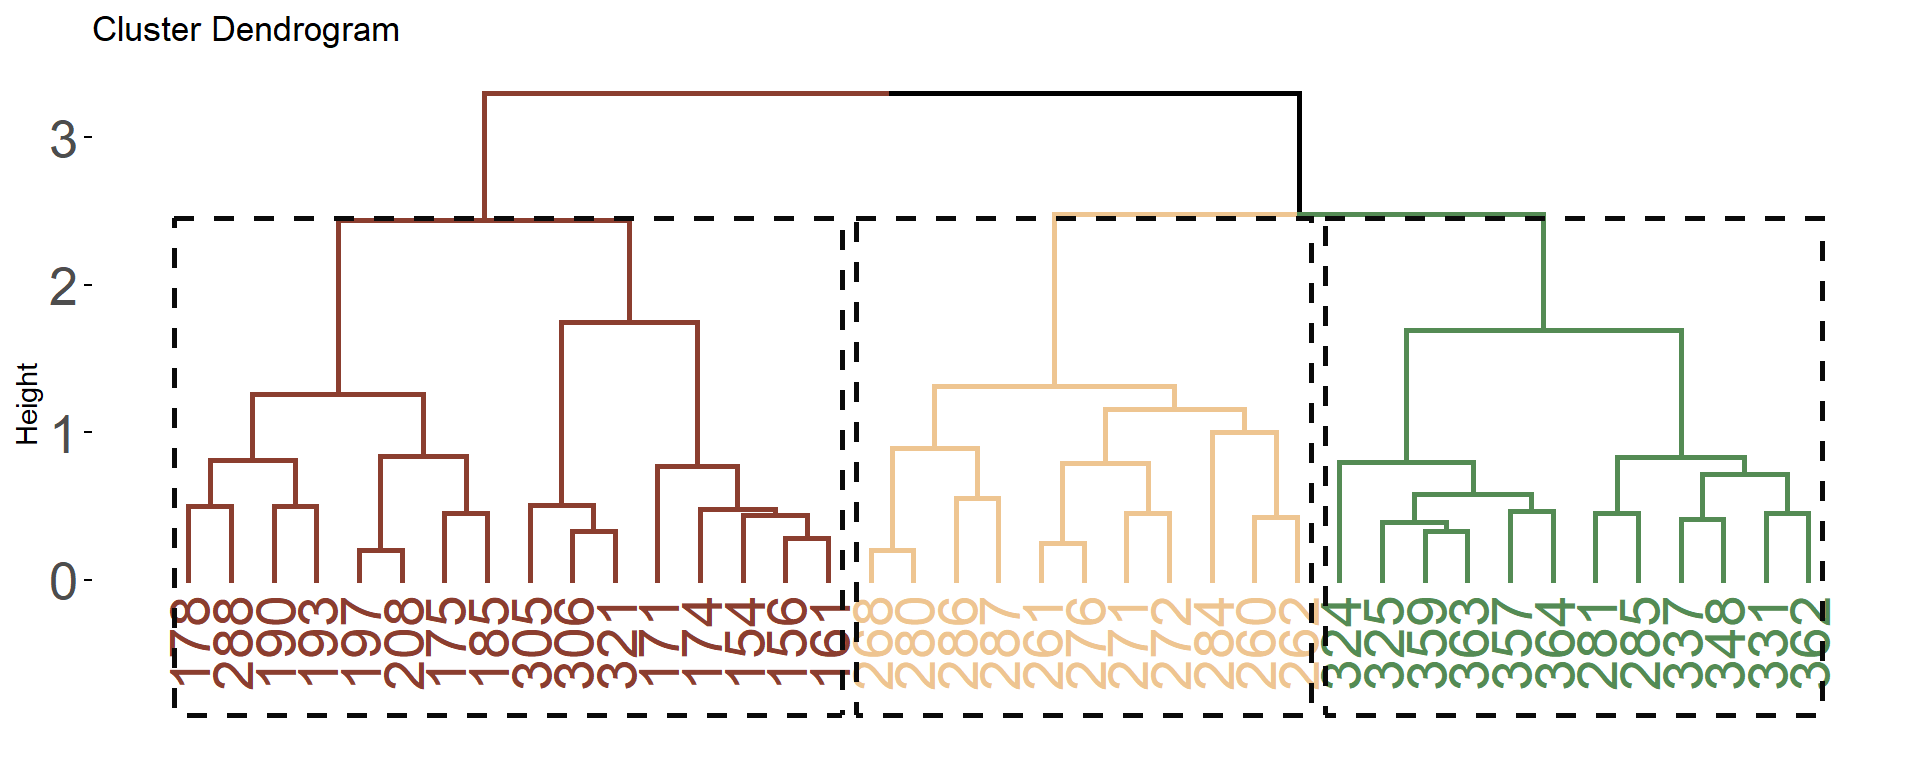
\includegraphics[width=0.95\linewidth]{madAcids_files/figure-latex/unnamed-chunk-60-1} \end{center}

\begin{itemize}
\tightlist
\item
  Correlaciones: Se evidenciaron relaciones lineales entre los ácidos
  orgánicos, entre el ácido málico y el ácido quínico con un coeficiente
  de correlación (r) de 0.8600213 y un valor de p=0.000333, y entre el
  ácido tartárico y el ácido succínico con un r=0.6869819 y un
  p-valor=0.01358. La acidez titulable total (TTA) mostró una asociación
  lineal significativa únicamente con el ácido tartárico, con un
  r=-0.7187027 y un p-valor=0.00845. Sin embargo, esta asociación
  inversa está vinculada al hecho de que el ácido tartárico solo aparece
  en cantidades mínimas en frutas muy maduras. La concentración total de
  ácidos con ácido quínico presentó una correlación de 0.8557676 con un
  p-valor=0.0003839. Mientras tanto, el ácido málico mostró un
  r=0.9300893 y un p-valor=1.169e-05. En ambos casos, estos ácidos
  explican el aumento en la concentración total de ácidos a lo largo del
  proceso de maduración de la fruta.
\end{itemize}

\end{document}
